\documentclass[a4paper,8pt]{article}
\usepackage{vntex}
\usepackage[english]{babel}
\usepackage[utf8]{inputenc}
\usepackage{ragged2e}
\usepackage{indentfirst}
\usepackage{graphicx}
\graphicspath{{./}{image/}{report/}{report/image/}}
\usepackage{float}
\usepackage{titlesec}
\usepackage{multirow}
\usepackage{multicol}
\usepackage{csvsimple}
% Giảm kích thước của các tiêu đề
\titleformat{\section}{\Large\bfseries}{\thesection}{1em}{}
\titleformat{\subsection}{\Large\bfseries}{\thesubsection}{1em}{}
\titleformat{\subsubsection}{\Large\bfseries}{\thesubsubsection}{1em}{}

\makeatletter
\renewcommand{\numberline}[1]{%
  \settowidth{\dimen0}{#1\quad}%
  \ifdim\dimen0>\@tempdima
    \hb@xt@\dimen0{#1\hfil}%
  \else
    \hb@xt@\@tempdima{#1\hfil}%
  \fi
}
\makeatother


\usepackage{xcolor} % Hỗ trợ màu sắc
\usepackage{listings} % Gói hiển thị mã nguồn

\lstset{
    language=Python, % Ngôn ngữ là Python
    basicstyle=\ttfamily\small, % Kiểu chữ và kích thước
    keywordstyle=\color{blue}, % Màu cho từ khóa
    frame=single, % Tạo khung quanh mã
    numbers=left, % Đánh số dòng bên trái
    numberstyle=\tiny\color{gray}, % Kiểu số dòng
    breaklines=true, % Tự động xuống dòng
    tabsize=2 % Kích thước tab
}
\usepackage{hyperref} % Gói tạo liên kết nội bộ
\usepackage{fancyhdr}
\usepackage{tabularx}
\usepackage{amsmath}
\usepackage{amssymb}
\usepackage{lastpage}
\usepackage[headheight=2cm, headsep=1.5cm]{geometry}
\usepackage{tikz}
\usetikzlibrary{shapes.geometric, arrows, positioning}
\tikzstyle{startstop} = [rectangle, rounded corners, minimum width=3cm, minimum height=1cm,text centered, draw=black, fill=white]
\tikzstyle{process} = [rectangle, minimum width=3cm, minimum height=1cm, text centered, draw=black, fill=white]
\tikzstyle{decision} = [diamond, minimum width=3cm, minimum height=1cm, text centered, draw=black, fill=white]
\tikzstyle{arrow} = [thick,->,>=stealth]
\pagestyle{fancy}
\fancyhf{}
\fancyhead[L]{
 \begin{tabular}{rl}
    \begin{picture}(25,15)(0,0)
    \put(0,-8){
\includegraphics[width=8mm, height=8mm]{image/hcmut.jpg}}
    %\put(0,-8){\epsfig{width=10mm,figure=hcmut.eps}}
   \end{picture}&
	%\includegraphics[width=8mm, height=8mm]{image/hcmut.png} & %
	\begin{tabular}{l}
		\textbf{\bf \ttfamily Ho Chi Minh City University of Technology}\\
		\textbf{\bf \ttfamily Faculty of Computer Science and Engineering}
	\end{tabular}
 \end{tabular}
}

\fancyfoot[L]{\scriptsize \ttfamily Instructor: Dr. Lê Thành Sách}
\fancyfoot[R]{\scriptsize \ttfamily Page {\thepage}/\pageref{LastPage}}
\renewcommand{\headrulewidth}{0.3pt}
\renewcommand{\footrulewidth}{0.3pt}

\begin{document}
\begin{titlepage}
\thispagestyle{empty}
\centering

\vspace*{0.8cm}
{\small
Vietnam National University, Ho Chi Minh City\\
University of Technology\\
Faculty of Computer Science and Engineering
}

\vspace{1.2cm}

\includegraphics[width=2.8cm]{image/hcmut.jpg}

\vspace{1.1cm}
{\large\textbf{Assignment}}\\[0.15cm]
{\LARGE\textbf{Plant Disease Localization and}}\\[0.1cm]
{\LARGE\textbf{Classification on Field Images}}

\vspace{0.8cm}
\rule{0.82\textwidth}{0.5pt}

\vspace{0.65cm}
{\Large\textbf{Programming Foundation for Data Analytics and Visualization}}

\vspace{0.65cm}
\rule{0.82\textwidth}{0.5pt}

\vspace{0.8cm}
{\Large\textbf{Instructor: Dr. Lê Thành Sách}}

\vspace{0.3cm}
\begin{tabular}{rll}
\textbf{Sinh viên thực hiện}: & Nguyễn Lâm Huy & 2311188\\
& Nguyễn Tất Kiên & 2311735\\
& Nguyễn Thành Minh Khôi & 2311687
\end{tabular}

\vfill
{\small\today}
\vspace*{0.8cm}

\end{titlepage}
\section*{Duty Roster}
\addcontentsline{toc}{section}{Member list \& Workload}
\begin{center}
\begin{table}[h]
\centering
\small
\renewcommand{\arraystretch}{1.15}
\begin{tabularx}{\textwidth}{|c|>{\centering\arraybackslash}X|c|>{\raggedright\arraybackslash}X|c|}
\hline
\textbf{No.} & \textbf{Name} & \textbf{StuID} & \textbf{Work} & \textbf{\% Progress}\\
\hline
1 & Nguyễn Tất Kiên & 2311735 & Image Part Assignment & 100\%\\
\hline
2 & Nguyễn Thành Minh Khôi & 2311687 & Tabular Part Assignment & 100\%\\
\hline
3 & Nguyễn Lâm Huy & 2311188 & Text Part Assignment & 100\%\\
\hline
\end{tabularx}
\end{table}
\end{center}

\clearpage
\tableofcontents
\clearpage

\section{Introduction}

Automatic recognition of plant disease from photographs is usually presented as an image
classification problem, but field photographs may contain several overlapping plants, soil,
shadows, and visually similar background vegetation. The task must therefore identify both the
region being described and its disease or health state.

This report studies the problem in its two-level form. Given a field photograph, the system
must first \emph{localize} each annotated plant region and then \emph{classify} its disease or
health state. The two stages are evaluated separately because a missed region never reaches the
classifier, whereas a correctly localized region may still be mislabelled.

\subsection{Objectives}

The objectives are to characterize FieldPlant, build a classical colour-and-morphology baseline,
train the Ultralytics YOLO26n detector~\cite{yolo26} on the same split, and compare both tracks
under one matching protocol.

\subsection{Contributions}

The report quantifies class imbalance and the limits of colour-based localization, evaluates six
proposal configurations, two feature representations, and ten classifier candidates, and
compares the selected classical pipeline with class-aware YOLO26n. Its attribution analysis
shows that localization coverage explains most of the performance gap.

\section{Dataset and Experimental Protocol}
\label{sec:dataset}

\subsection{Source and acquisition}

All experiments use FieldPlant~\cite{fieldplant}, a public collection of plantation photographs
with plant-region bounding boxes, released through Roboflow Universe~\cite{roboflow}. The study
uses a YOLO-format export of that release.

The export used here contains \textbf{5{,}156 images} and \textbf{8{,}580 annotated boxes}
distributed over \textbf{27 classes}: five cassava, sixteen corn, and six tomato states. Because
the export places every image in one directory, the notebook constructs the validation and test
partitions.

\subsection{Image-level stratified split}

Images, rather than individual boxes, are split so that all annotations from one photograph stay
together. Majority-class stratification produces a \textbf{70\,/\,15\,/\,15} train,
validation, and test split. Corn Charcoal and Tomato bacterial wilt are pinned to training
because their support is too small for stratification; Table~\ref{tab:split} gives the outcome.

\begin{table}[H]
\centering
\small
\renewcommand{\arraystretch}{1.2}
\begin{tabularx}{0.82\textwidth}{|l|r|r|>{\raggedright\arraybackslash}X|}
\hline
\textbf{Partition} & \textbf{Images} & \textbf{Boxes} & \textbf{Role}\\
\hline
Train & 3{,}609 & 5{,}997 & Fits every model, scaler, PCA basis, and sampling tier\\
\hline
Validation & 773 & 1{,}318 & Selects proposal method, features, and classifier\\
\hline
Test & 774 & 1{,}265 & Evaluated once, for the selected configuration only\\
\hline
\textbf{Total} & \textbf{5{,}156} & \textbf{8{,}580} & \\
\hline
\end{tabularx}
\caption{Image-level 70\,/\,15\,/\,15 split actually materialized by the notebook. Boxes follow
their parent image file, so the box proportions deviate slightly from 70\,/\,15\,/\,15.}
\label{tab:split}
\end{table}

\subsection{Integrity audit}

An independent parser verifies all \textbf{5{,}156 images} and \textbf{8{,}580 annotation rows}.
No image fails to decode, and no annotation has an unknown class, invalid coordinate, or
degenerate box.

\subsection{Evaluation discipline}

The refreshed exploratory analysis and earlier modelling run use the same materialized split,
verified by content signatures, but were not executed in one continuous run.

Four rules are enforced throughout and are the reason several quantities in this report are
lower than they would otherwise appear.

\begin{enumerate}
\item \textbf{Train-only fitting.} Every quantity estimated from data is estimated on the
training partition alone. This includes the \texttt{StandardScaler} used by the linear
classifiers, the PCA basis used in Section~\ref{sec:pca}, the class-frequency counts that
produce the balanced class weights, and the oversampling tiers of
Section~\ref{sec:yolo-method}. Validation and test features are transformed by these fitted
objects, never used to fit them.
\item \textbf{Validation selects, test confirms.} The proposal configuration, the feature
representation, and the classifier hyperparameters are chosen using validation results only.
The test partition is evaluated once, for the selected configuration.
\item \textbf{No augmentation or oversampling outside training.} Augmentation transforms and
repeated-path manifests apply exclusively to training images. Validation and test directories
are never modified. The notebook verifies this by comparing content signatures of those
directories before and after training.
\item \textbf{Fixed seeds.} A single seed, $42$, governs the split, the class-capped feature
sampling, the classifier initializations, and the detector training run, and the detector is
trained in deterministic mode.
\end{enumerate}

\section{Exploratory Data Analysis}
\label{sec:eda}

SHA-256 comparison finds \textbf{113 groups of byte-identical files spanning
partitions}. This leakage makes held-out results optimistic by an unknown amount; the split is
left unchanged for reproducibility, and Section~\ref{sec:limitations} records the consequence.
Hashing detects exact duplicates only, not recompressed or near-duplicate photographs.

\subsection{Class imbalance and evaluation coverage}
\label{sec:imbalance}

\begin{figure}[H]
\centering
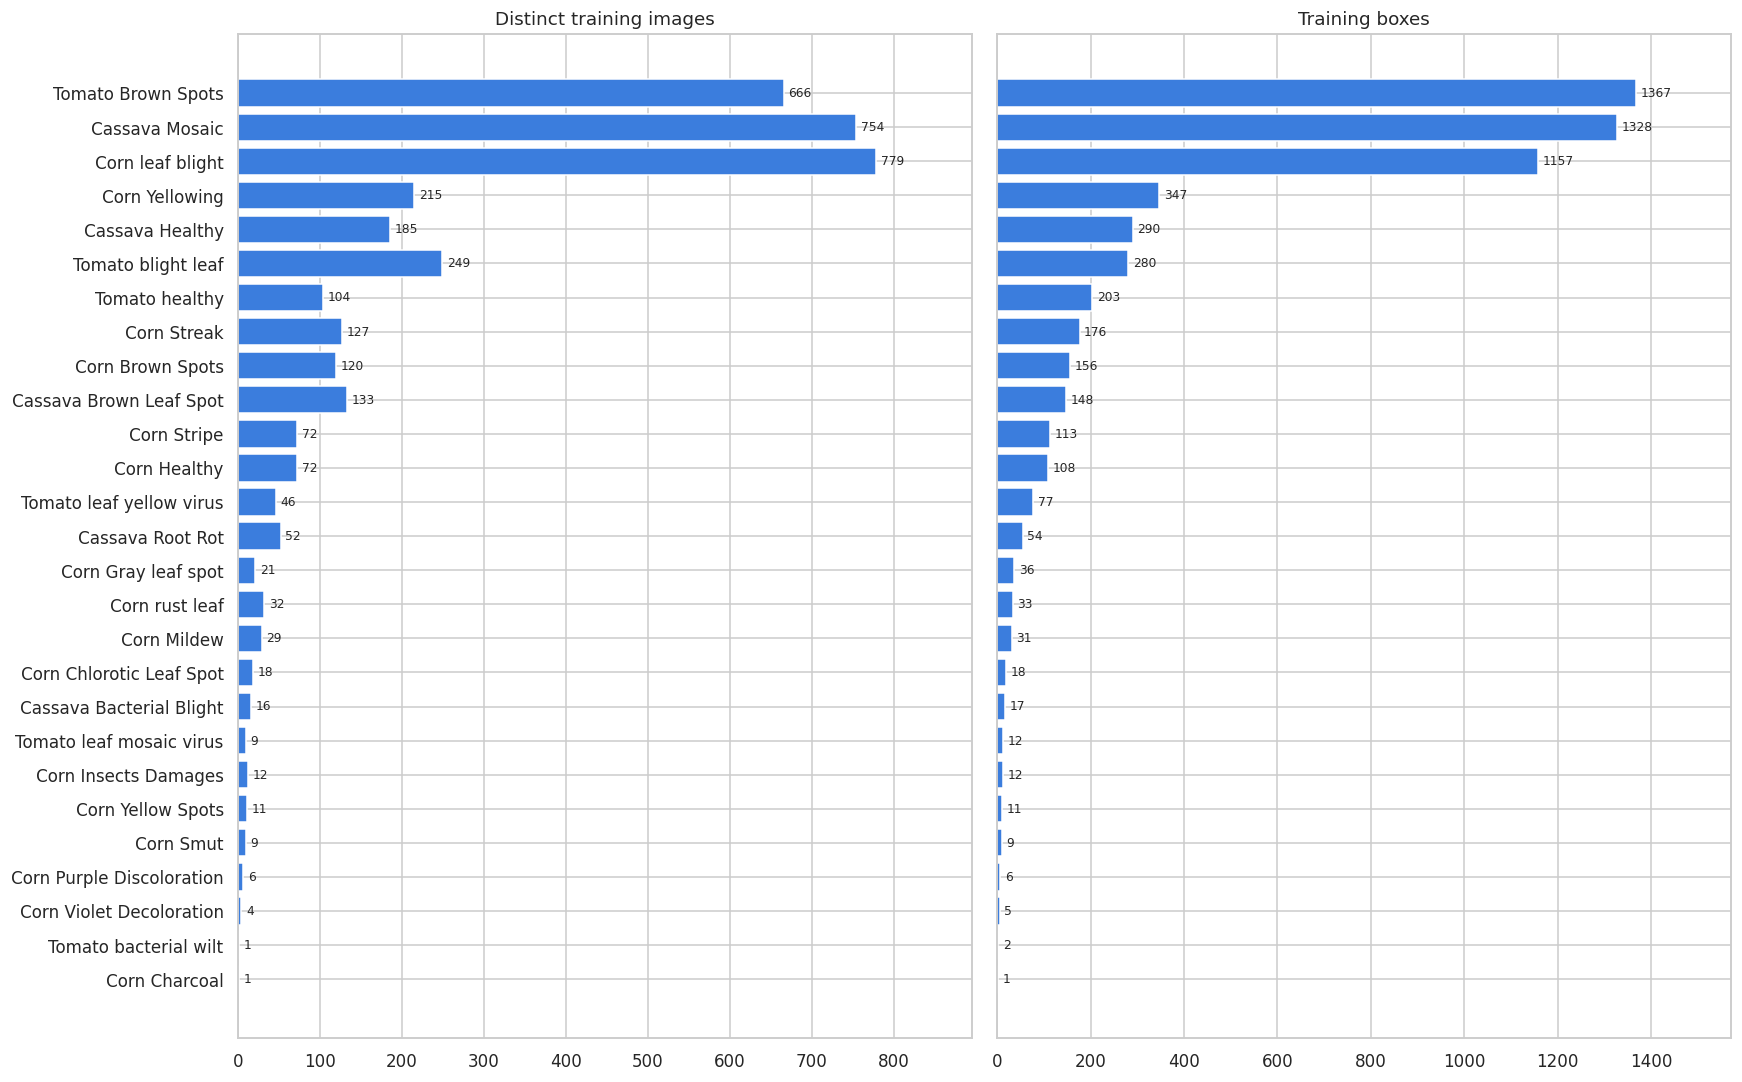
\includegraphics[width=\textwidth]{image/class_distribution.png}
\caption{Distinct training images (left) and training boxes (right) for each of the 27 classes,
sorted by box count. The two panels share a vertical axis, so the horizontal difference between
them shows how many boxes a class contributes per photograph.}
\label{fig:class-distribution}
\end{figure}

Figure~\ref{fig:class-distribution} shows a distribution that is not merely skewed but skewed
across three orders of magnitude. The three largest classes, Tomato Brown Spots with 1{,}367
training boxes, Cassava Mosaic with 1{,}328, and Corn leaf blight with 1{,}157, together hold
3{,}852 of the 5{,}997 training boxes, that is \textbf{64.2\%} of the training annotations. At
the other end, \textbf{ten of the 27 classes have fewer than 20 training boxes}, and the
smallest, Corn Charcoal, has a single box in a single photograph.

The imbalance also determines what can be measured. Table~\ref{tab:class-coverage} gives the
per-class box counts in each partition. Two classes, \textbf{Corn Charcoal} and \textbf{Tomato
bacterial wilt}, have no boxes at all in validation or test. For these two classes the report
can describe training behaviour but cannot report held-out performance of any kind, and any
per-class metric printed for them is an artefact of the averaging convention rather than a
measurement. Several further classes, such as Corn Purple Discoloration and Corn Violet
Decoloration with one validation box each, are technically evaluable but their per-class scores
are determined by a single detection.

\begin{table}[H]
\centering
\scriptsize
\renewcommand{\arraystretch}{1.08}
\begin{tabularx}{0.95\textwidth}{|X|r|r|r||X|r|r|r|}
\hline
\textbf{Class} & \textbf{Tr} & \textbf{Va} & \textbf{Te} &
\textbf{Class} & \textbf{Tr} & \textbf{Va} & \textbf{Te}\\
\hline
Cassava Bacterial Blight & 17 & 5 & 3 & Corn Streak & 176 & 35 & 41\\
Cassava Brown Leaf Spot & 148 & 34 & 29 & Corn Stripe & 113 & 25 & 24\\
Cassava Healthy & 290 & 70 & 57 & Corn Violet Decoloration & 5 & 1 & 1\\
Cassava Mosaic & 1{,}328 & 285 & 284 & Corn Yellow Spots & 11 & 3 & 2\\
Cassava Root Rot & 54 & 11 & 12 & Corn Yellowing & 347 & 75 & 73\\
Corn Brown Spots & 156 & 31 & 33 & Corn leaf blight & 1{,}157 & 256 & 239\\
Corn Charcoal & 1 & 0 & 0 & Corn rust leaf & 33 & 7 & 9\\
Corn Chlorotic Leaf Spot & 18 & 4 & 4 & Tomato Brown Spots & 1{,}367 & 298 & 302\\
Corn Gray leaf spot & 36 & 10 & 8 & Tomato bacterial wilt & 2 & 0 & 0\\
Corn Healthy & 108 & 25 & 19 & Tomato blight leaf & 280 & 62 & 62\\
Corn Insects Damages & 12 & 3 & 2 & Tomato healthy & 203 & 43 & 33\\
Corn Mildew & 31 & 6 & 6 & Tomato leaf mosaic virus & 12 & 4 & 3\\
Corn Purple Discoloration & 6 & 1 & 1 & Tomato leaf yellow virus & 77 & 22 & 16\\
Corn Smut & 9 & 2 & 2 & \textbf{Total} & \textbf{5{,}997} & \textbf{1{,}318} & \textbf{1{,}265}\\
\hline
\end{tabularx}
\caption{Annotated boxes per class and partition. Classes are listed in the order defined by the
dataset. The two rows with zero validation and test boxes cannot be evaluated on held-out data.}
\label{tab:class-coverage}
\end{table}

Because boxes from one photograph are correlated and the three largest classes dominate the
counts, the report uses macro-$F_1$ with per-class support and reweights or resamples training.

\subsection{Objects per image}
\label{sec:objects-per-image}

\begin{figure}[H]
\centering
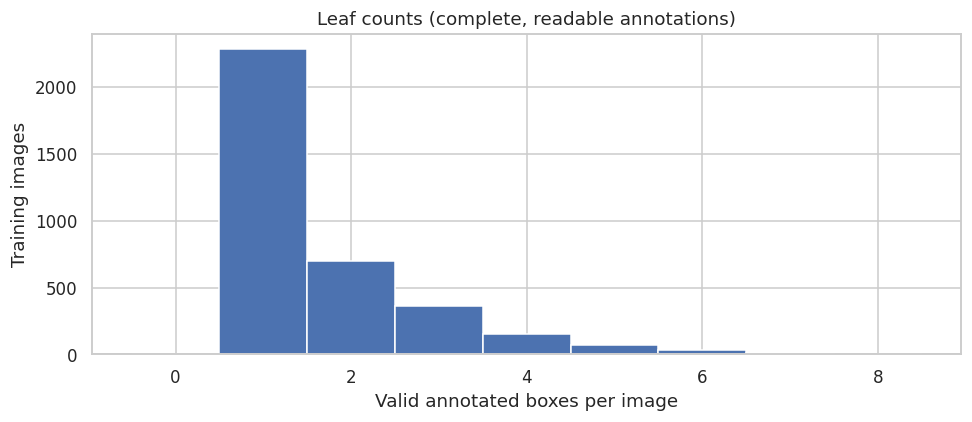
\includegraphics[width=0.72\textwidth]{image/leaf_counts.png}
\caption{Number of valid annotated boxes per training photograph, over the 3{,}609 images with
complete and readable annotations.}
\label{fig:leaf-counts}
\end{figure}

Figure~\ref{fig:leaf-counts} answers a question that constrains the classical pipeline directly.
Across the 3{,}609 eligible training images, \textbf{63.3\% contain exactly one annotated
object}, \textbf{36.7\% contain more than one}, and \textbf{17.5\% contain more than two}. No
eligible image has zero boxes.

The classical proposal stage of Section~\ref{sec:classical-method} retains at most two boxes per
image. Using Equation~\eqref{eq:ceiling} with $k=2$ and assuming perfect box placement, it could
match at most \textbf{82.3\%} of the training annotations: images with three or more objects
necessarily lose the remainder. This count-only bound isolates the retention rule from mask
quality; detectors without a two-box limit retain a structural advantage on multi-object images.

\subsection{Box geometry and scale}
\label{sec:geometry}

Detector and classifier input sizes are only meaningful relative to the size of the objects.
Table~\ref{tab:geometry} summarizes the geometry of the 5{,}997 training boxes in three forms:
their size in original pixels, their physical aspect ratio, and their \emph{nominal} size after
an aspect-preserving resize of the photograph to a 640-pixel long side, which is the input
convention used by the detector.

\begin{table}[H]
\centering
\small
\renewcommand{\arraystretch}{1.15}
\begin{tabularx}{0.95\textwidth}{|>{\raggedright\arraybackslash}X|r|r|r|r|r|r|}
\hline
\textbf{Quantity} & \textbf{Min} & \textbf{5\%} & \textbf{Median} & \textbf{Mean} & \textbf{95\%} & \textbf{Max}\\
\hline
Box width (px) & 78.2 & 525.2 & 1{,}476.0 & 1{,}688.4 & 3{,}398.7 & 4{,}608.0\\
\hline
Box height (px) & 57.5 & 519.0 & 1{,}580.0 & 1{,}875.3 & 4{,}158.0 & 4{,}608.0\\
\hline
Aspect ratio (width\,/\,height) & 0.10 & 0.39 & 0.92 & 1.08 & 2.22 & 6.33\\
\hline
Nominal short side (px) & 11.8 & 88.3 & 219.3 & 247.3 & 472.5 & 639.3\\
\hline
\end{tabularx}
\caption{Distribution of training box geometry. ``Nominal short side'' is the shorter box
dimension after an aspect-preserving resize of the photograph to a 640-pixel long side.}
\label{tab:geometry}
\end{table}

The annotations are large. The median box occupies a substantial part of its photograph, and at
the nominal 640-pixel working resolution the median box still has a short side of
\textbf{219.3 pixels}. Only \textbf{0.02\%} of boxes fall below a 16-pixel short side and
\textbf{0.08\%} below 32 pixels. Small-object detection is therefore not the binding constraint here. These nominal sizes
ignore letterboxing, rounding, and augmentation, and boxes can overstate the extent of
non-rectangular plant tissue.

Aspect ratio is a different matter. The central 90\% of boxes span ratios from 0.39 to 2.22 and
the extremes reach 0.10 and 6.33, meaning some annotations are roughly ten times taller than
they are wide. Because the classical classifier resizes every crop to a fixed
$128 \times 128$ square, such boxes are geometrically distorted before any feature is computed.

\subsection{Spatial distribution of annotations}

\begin{figure}[H]
\centering
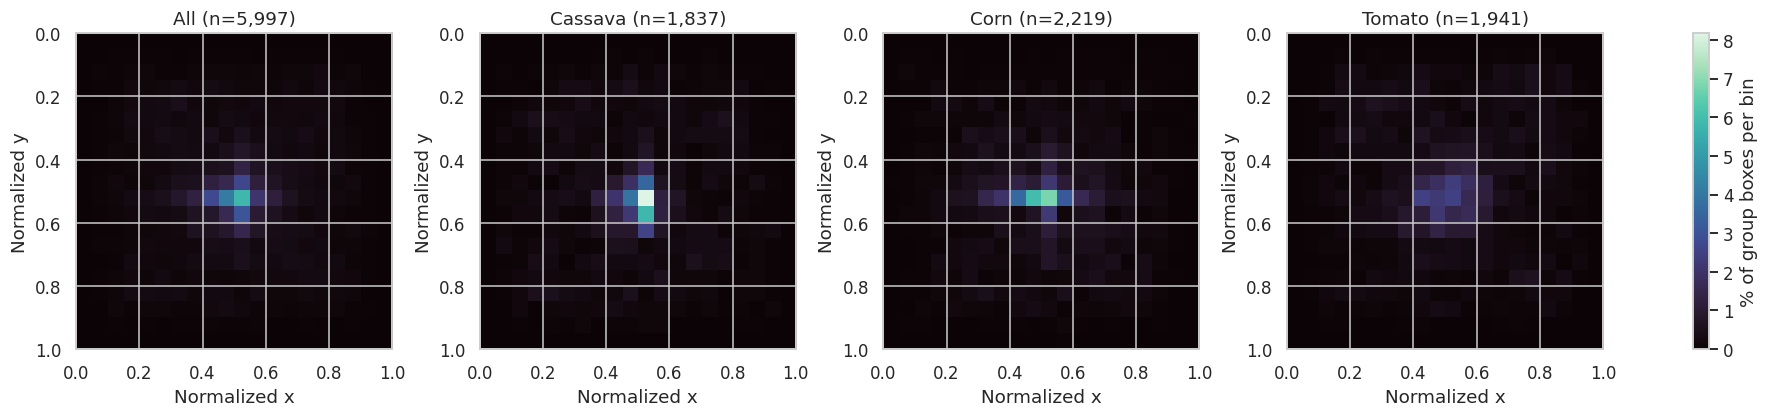
\includegraphics[width=\textwidth]{image/box_center_heatmap.png}
\caption{Normalized annotation centres over the training partition: all boxes, then cassava,
corn, and tomato separately. Each cell reports the percentage of that group's boxes, on a shared
colour scale. The vertical axis increases downwards, matching image coordinates.}
\label{fig:center-heatmap}
\end{figure}

Figure~\ref{fig:center-heatmap} shows that annotation centres are strongly concentrated:
\textbf{65.6\% of training box centres fall inside the central quarter of the image area},
defined as the region where both normalized coordinates lie in $[0.25, 0.75]$. The
concentration is sharpest for cassava and corn. Tomato centres are visibly more dispersed, which
is consistent with tomato photographs containing several annotated regions more often.

This pattern is a statement about how the corpus was photographed and annotated. The
photographer aimed at the plant of interest and the annotator labelled it, so the label lands
near the centre. It does not follow that diseased plants occur near image centres in general,
and a model that learned a centre prior would be learning a property of the acquisition process.
Error inspection therefore includes off-centre and border-touching objects.

\subsection{Classes that occur together}
\label{sec:cooccurrence}

\begin{figure}[H]
\centering
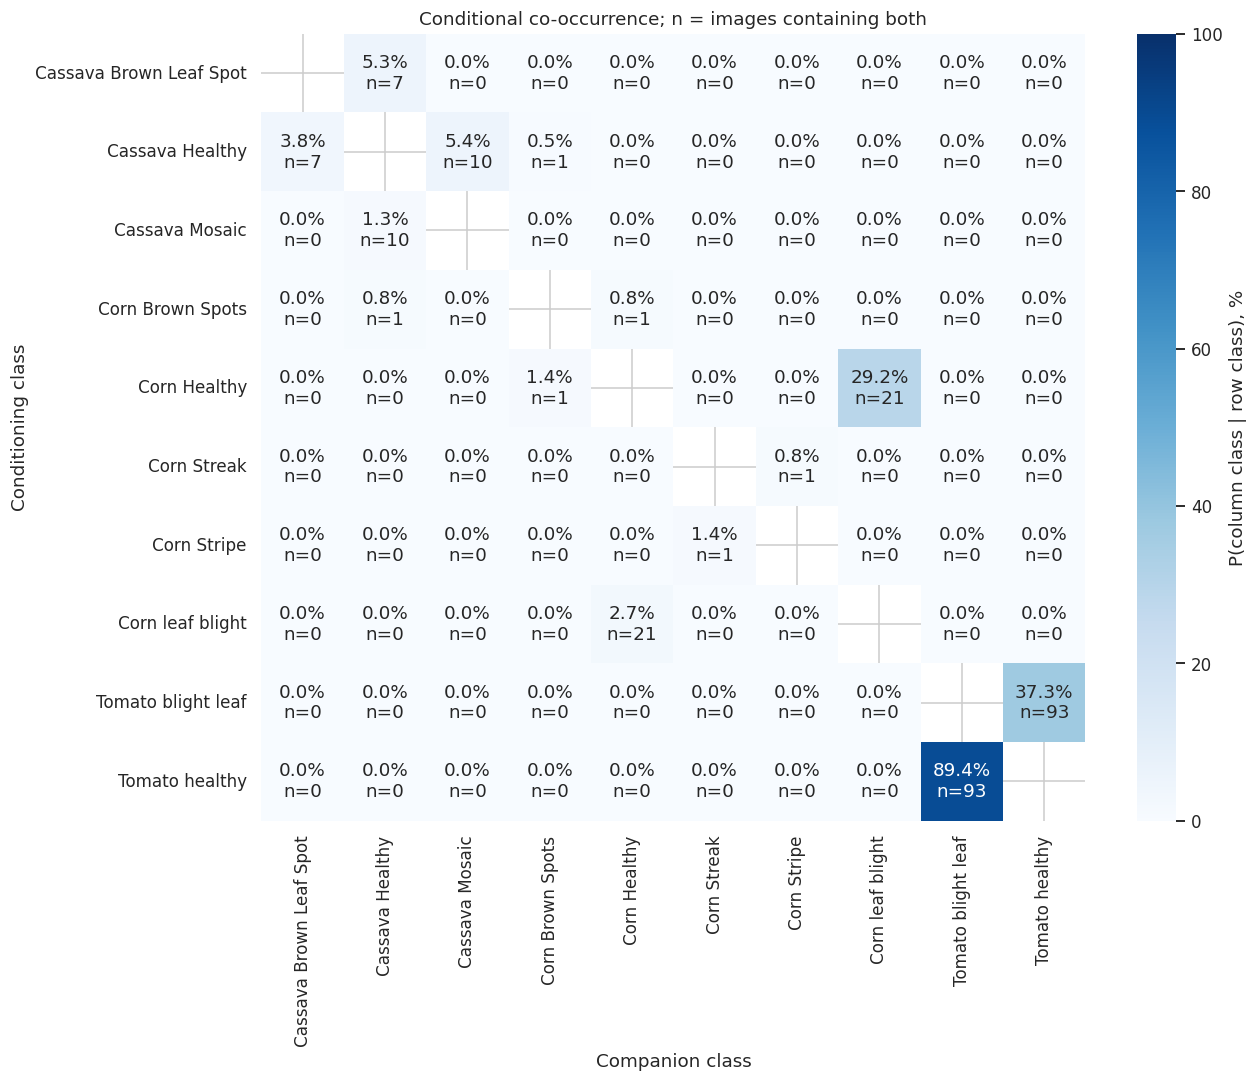
\includegraphics[width=0.78\textwidth]{image/class_cooccurrence.png}
\caption{Conditional co-occurrence for class pairs found in the same training photograph. Cell
$(a,b)$ reports the percentage of training photographs of the row class that also contain the
column class, together with the supporting image count. The matrix is asymmetric and the
diagonal is masked.}
\label{fig:cooccurrence}
\end{figure}

Only \textbf{seven distinct class pairs} ever appear together in a training photograph, and
Table~\ref{tab:cooccurrence} lists all of them. The relationship is dominated by a single pair:
\textbf{93 photographs contain both Tomato healthy and Tomato blight leaf}, which is exactly the
situation one expects when a diseased and a healthy leaf of the same plant appear in one frame.

Because Figure~\ref{fig:cooccurrence} is conditional, direction matters. Those same 93 images
constitute \textbf{89.4\% of the photographs containing Tomato healthy} but only \textbf{37.3\%
of those containing Tomato blight leaf}. Reading the matrix symmetrically would therefore
misstate the relationship in one of the two directions. Three of the seven pairs rest on a
single photograph each, and one of them, Cassava Healthy together with Corn Brown Spots, crosses
crop boundaries and is worth inspecting as a possible annotation error rather than treated as a
real biological co-occurrence.

\begin{table}[H]
\centering
\small
\renewcommand{\arraystretch}{1.15}
\begin{tabularx}{0.9\textwidth}{|>{\raggedright\arraybackslash}X|>{\raggedright\arraybackslash}X|r|}
\hline
\textbf{Class A} & \textbf{Class B} & \textbf{Images}\\
\hline
Tomato blight leaf & Tomato healthy & 93\\
\hline
Corn Healthy & Corn leaf blight & 21\\
\hline
Cassava Healthy & Cassava Mosaic & 10\\
\hline
Cassava Brown Leaf Spot & Cassava Healthy & 7\\
\hline
Cassava Healthy & Corn Brown Spots & 1\\
\hline
Corn Brown Spots & Corn Healthy & 1\\
\hline
Corn Streak & Corn Stripe & 1\\
\hline
\end{tabularx}
\caption{All class pairs co-occurring in at least one training photograph.}
\label{tab:cooccurrence}
\end{table}

Co-occurrence supported by one or two photographs is unstable and does not validate the
annotations. It nevertheless confirms that splitting by image is mandatory; cross-crop pairs
also warrant manual inspection.

\subsection{Representative photographs and classifier inputs}

\begin{figure}[H]
\centering
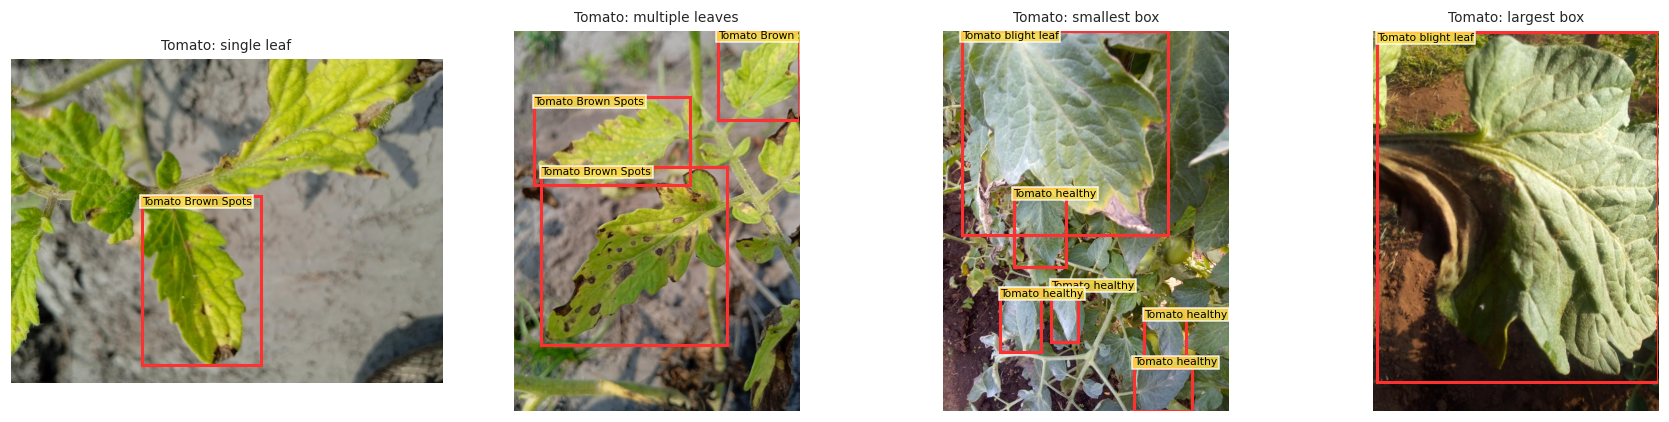
\includegraphics[width=\textwidth]{image/tomato_samples.png}
\caption{Four tomato training photographs with ground-truth boxes in red: one annotated leaf,
several annotated leaves, the smallest tomato annotation, and the largest.}
\label{fig:tomato-samples}
\end{figure}

Figure~\ref{fig:tomato-samples} is included to prevent a misleading mental image of the corpus.
A single representative photograph does not exist: the same class appears as one clean,
well-separated leaf, as a cluster of overlapping leaves each carrying its own annotation, as a
small local region inside a wider scene, and as an object filling almost the whole frame. Any
localization heuristic tuned on the first case will not transfer to the second.

Inspecting one or two original crops from every class also surfaces a scope question. The crops
displayed for \textbf{Corn Charcoal} and \textbf{Corn Smut} include ears and tassels rather than
leaf blades alone, so the annotations are not restricted to leaves even though the task is
frequently described in those terms. A montage cannot establish how often this happens, and no
annotation was removed on the strength of it. The point is recorded so that the task definition
used in Section~\ref{sec:method} speaks of plant regions rather than leaves. One further record
was found in which annotations of two different crops, cassava and corn, occur in the same
photograph. These examples also motivate including crowded scenes in qualitative evaluation.

\subsection{Structure of the handcrafted feature space}
\label{sec:pca}

\begin{figure}[H]
\centering
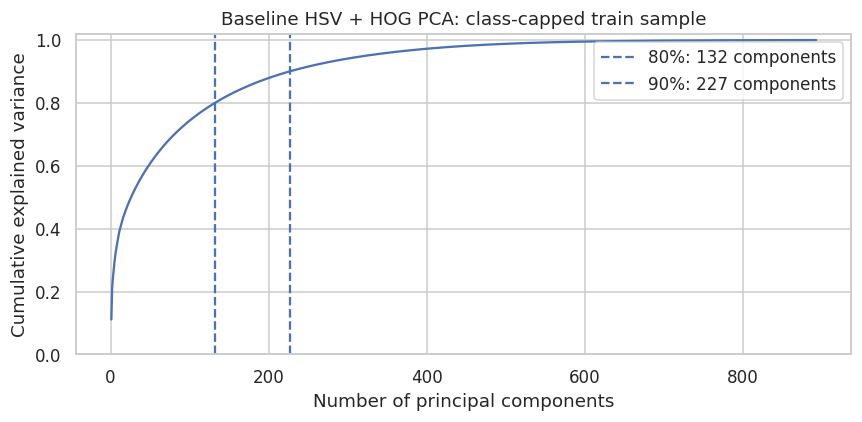
\includegraphics[width=0.72\textwidth]{image/pca_cumulative_variance.png}
\caption{Cumulative explained variance of a PCA fitted to standardized HSV and HOG features of
class-capped training crops.}
\label{fig:pca}
\end{figure}

To understand what the classical representation offers before any classifier is fitted, the
baseline 1{,}812-dimensional HSV and HOG descriptor of Section~\ref{sec:features} is computed on
a class-capped training sample of at most 50 crops per class, yielding \textbf{893 usable
crops} from 783 photographs, and a PCA is fitted to the standardized result.

Figure~\ref{fig:pca} shows that the representation is genuinely high dimensional. The first two
principal components retain only \textbf{21.2\%} of the variance. Reaching 80\% requires
\textbf{132 components} and reaching 90\% requires \textbf{227}. The practical consequence is
about interpretation rather than about modelling. A two-dimensional scatter plot of the first two
components shows less than a quarter of the variation, so classes that overlap in that
projection have not been shown to be inseparable. They have only been shown to be
indistinguishable in a projection that discards four fifths of the signal.

PCA measures variance rather than class separation and depends on the standardized, class-capped
sample. Low-dimensional projections are therefore used for inspection only; separability claims
come from held-out classifier metrics.

\subsection{Feasibility of colour-based localization}
\label{sec:proposal-probe}

The classical track localizes objects by colour and morphology, so its feasibility should be
probed before it is built in full. The probe applies the same Excess Green and HSV filtering
pipeline and the same top-two retention rule used later, on 100 seeded training photographs
containing 153 annotated objects, and matches proposals to annotations with the greedy procedure
of Section~\ref{sec:localization-metrics}.

\begin{figure}[H]
\centering
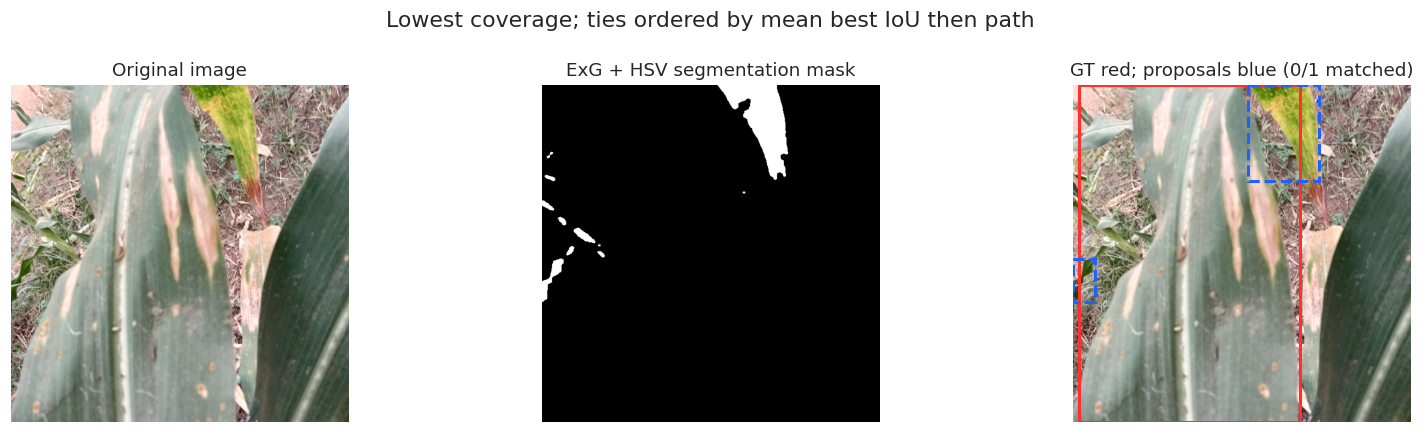
\includegraphics[width=\textwidth]{image/exg_hsv_low_coverage.png}
\caption{A low-coverage example. Left to right: the photograph with the red ground-truth box,
the vegetation mask, and the retained proposals in blue. Discoloration and background foliage
fragment the mask, and no retained proposal reaches an IoU of 0.5 with the annotation.}
\label{fig:exg-low}
\end{figure}

\begin{figure}[H]
\centering
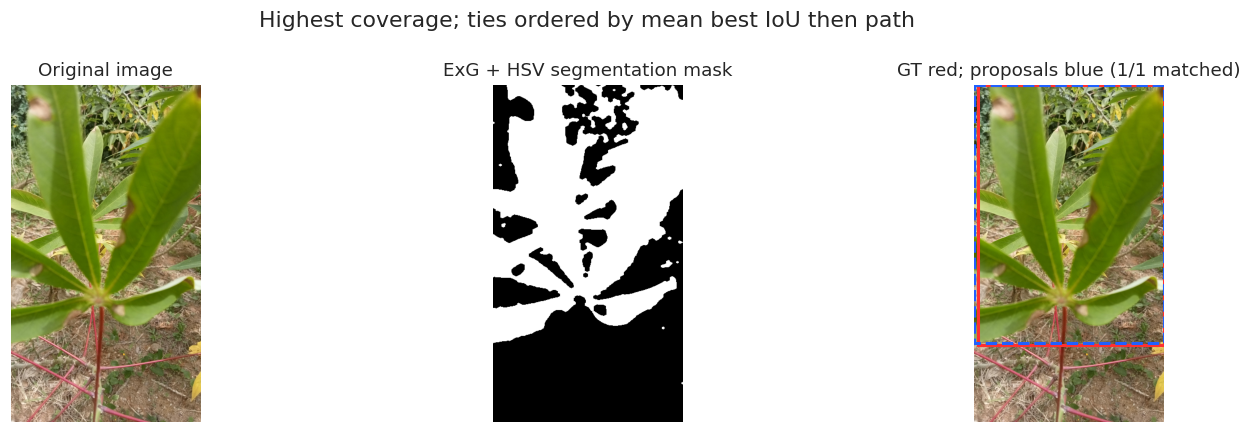
\includegraphics[width=\textwidth]{image/exg_hsv_high_coverage.png}
\caption{A high-coverage example. A clean green foreground against a contrasting background
yields one proposal that follows the ground-truth box closely.}
\label{fig:exg-high}
\end{figure}

The two examples show the mechanism in both directions. In Figure~\ref{fig:exg-high} the object
is a compact green region against a dissimilar background, the mask has one connected component,
and the fitted box nearly coincides with the annotation. In Figure~\ref{fig:exg-low} the leaf is
discoloured, which removes part of it from a green-based mask, while healthy background
vegetation is retained. The mask splits into fragments and the two largest of them describe
regions that the annotation does not.

Aggregated over the sample, the second behaviour is the common one. The procedure keeps 192
proposals, an average of 1.92 per photograph, and matches only \textbf{45 of the 153 annotated
objects}, a coverage of \textbf{29.4\%}, leaving \textbf{108 unmatched}. The mean best IoU per
annotation, as defined in Equation~\eqref{eq:meaniou}, is \textbf{0.375}, comfortably below the
0.5 matching threshold. In other words the typical proposal overlaps its nearest annotation
partially rather than either missing it entirely or capturing it.

This training-only probe is small, and mean best IoU is not one-to-one like coverage. It still
identifies localization as the expected bottleneck, motivating separate classification
measurements on annotation crops and proposal crops.

\section{Proposed Method}
\label{sec:method}

\subsection{Two-level architecture}

The classical track proposes regions using colour and morphology and then classifies their
crops; YOLO26n predicts boxes and classes jointly. The explicit separation permits stage-wise
attribution, while the shared matching stage in Figure~\ref{fig:pipeline} makes the final outputs
comparable.

\begin{figure}[H]
\centering
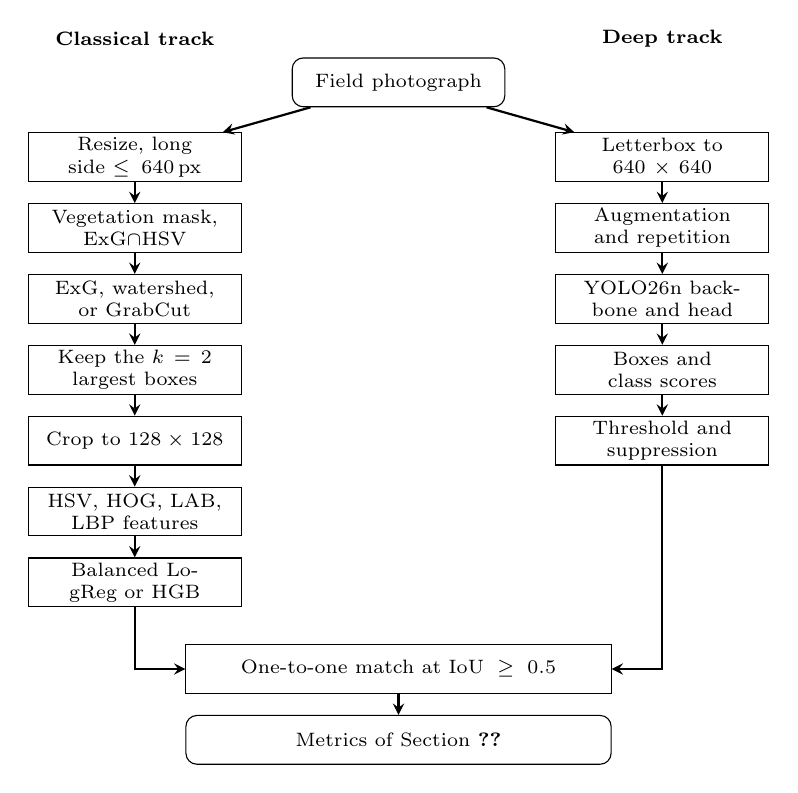
\begin{tikzpicture}[
  every node/.style={font=\scriptsize, inner sep=1.5pt},
  startstop/.append style={minimum width=2.7cm, minimum height=0.62cm},
  process/.append style={minimum width=2.7cm, minimum height=0.62cm, text width=2.6cm}
]

\node (img) [startstop] at (0,0) {Field photograph};

\node (c1) [process] at (-3.35,-0.95) {Resize, long side $\le 640$\,px};
\node (c2) [process] at (-3.35,-1.85) {Vegetation mask, $\mathrm{ExG}\cap$HSV};
\node (c3) [process] at (-3.35,-2.75) {ExG, watershed, or GrabCut};
\node (c4) [process] at (-3.35,-3.65) {Keep the $k=2$ largest boxes};
\node (c5) [process] at (-3.35,-4.55) {Crop to $128\times 128$};
\node (c6) [process] at (-3.35,-5.45) {HSV, HOG, LAB, LBP features};
\node (c7) [process] at (-3.35,-6.35) {Balanced LogReg or HGB};

\node (d1) [process] at (3.35,-0.95) {Letterbox to $640\times 640$};
\node (d2) [process] at (3.35,-1.85) {Augmentation and repetition};
\node (d3) [process] at (3.35,-2.75) {YOLO26n backbone and head};
\node (d4) [process] at (3.35,-3.65) {Boxes and class scores};
\node (d5) [process] at (3.35,-4.55) {Threshold and suppression};

\node (ev) [process, text width=5.2cm, minimum width=5.4cm] at (0,-7.45)
  {One-to-one match at $\mathrm{IoU}\ge 0.5$};
\node (mt) [startstop, minimum width=5.4cm] at (0,-8.35)
  {Metrics of Section~\ref{sec:metrics}};

\draw [arrow] (img) -- (c1);
\draw [arrow] (img) -- (d1);
\draw [arrow] (c1) -- (c2);
\draw [arrow] (c2) -- (c3);
\draw [arrow] (c3) -- (c4);
\draw [arrow] (c4) -- (c5);
\draw [arrow] (c5) -- (c6);
\draw [arrow] (c6) -- (c7);
\draw [arrow] (d1) -- (d2);
\draw [arrow] (d2) -- (d3);
\draw [arrow] (d3) -- (d4);
\draw [arrow] (d4) -- (d5);
\draw [arrow] (c7) |- (ev);
\draw [arrow] (d5) |- (ev);
\draw [arrow] (ev) -- (mt);

\node [font=\scriptsize\bfseries, inner sep=1pt] at (-3.35,0.55)
  {Classical track};
\node [font=\scriptsize\bfseries, inner sep=1pt] at (3.35,0.55)
  {Deep track};

\end{tikzpicture}
\caption{The two tracks and the shared evaluation stage. The classical track separates
localization from classification. YOLO26n performs both jointly. Both produce labelled boxes that
are matched against the annotations by the same procedure, which is what makes the comparison in
Section~\ref{sec:parity} meaningful.}
\label{fig:pipeline}
\end{figure}

\subsection{Shared preprocessing and constants}

Both tracks use RGB images and the split in Table~\ref{tab:split}. The fixed constants in
Table~\ref{tab:constants} ensure that configuration comparisons vary one factor at a time.

\begin{table}[H]
\centering
\small
\renewcommand{\arraystretch}{1.2}
\begin{tabularx}{0.95\textwidth}{|l|l|>{\raggedright\arraybackslash}X|}
\hline
\textbf{Constant} & \textbf{Value} & \textbf{Purpose}\\
\hline
\texttt{CROP\_SIZE} & $128 \times 128$ & Fixed square input of the classical classifier\\
\hline
\texttt{PROPOSAL\_LONG\_SIDE} & 640\,px & Working resolution of the proposal stage\\
\hline
\texttt{YOLO\_IMG\_SIZE} & 640\,px & Detector input size\\
\hline
\texttt{TOP\_K\_PROPOSALS} & 2 & Proposals retained per image after area ranking\\
\hline
\texttt{IOU\_MATCH} & 0.5 & IoU threshold of the matching protocol\\
\hline
\texttt{RANDOM\_STATE} & 42 & Split, sampling, initialization, and training seed\\
\hline
\end{tabularx}
\caption{Constants shared by both tracks.}
\label{tab:constants}
\end{table}

\subsection{Classical track}
\label{sec:classical-method}

\subsubsection{Vegetation mask}

The proposal stage assumes that plant tissue is distinguishable by colour. For RGB values
$R,G,B$, Excess Green is

\begin{equation}
\mathrm{ExG}(R,G,B) = 2G - R - B .
\label{eq:exg}
\end{equation}

The index is rescaled to $[0,255]$ and thresholded by Otsu's method. To reject greenish shadows
and soil, it is intersected with OpenCV HSV limits $25\le H\le95$, $S\ge25$, and $V\ge25$:

\begin{equation}
M_{\mathrm{green}} = \mathrm{Otsu}\!\left(\mathrm{ExG}\right) \;\wedge\;
\bigl[\, 25 \le H \le 95 \;\wedge\; S \ge 25 \;\wedge\; V \ge 25 \,\bigr],
\label{eq:greenmask}
\end{equation}

The mask receives one $5\times5$ elliptical opening and two closings to remove isolated pixels
and bridge small gaps.

\subsubsection{Guarded colour expansion}
\label{sec:expanded-mask}

Because diseased tissue may be yellow or brown, an expanded mask also considers yellow
($15\le H\le35$, $S,V\ge40$) and brown ($5\le H\le25$, $S\ge40$, $20\le V\le210$).
Discoloured pixels are retained when adjacent to an $11\times11$ dilation of the green mask, or
when a standalone component has area 0.2--50\%, aspect ratio at most 10, solidity at least 0.35,
and at most one border contact. The resulting expanded mask is denoted $M_{\mathrm{exp}}$.
One $3\times3$ opening and two $5\times5$ closings complete the
mask; the guards limit confusion with soil and litter.

\subsubsection{Region proposers}
\label{sec:proposers}

Three mechanisms convert a mask into boxes, and each is evaluated with both
$M_{\mathrm{green}}$ and $M_{\mathrm{exp}}$, giving six configurations.

\textbf{Excess Green and HSV} boxes external connected components directly. \textbf{Watershed}
separates touching components using distance-transform seeds above $0.35$ of the maximum and a
twice-dilated $3\times3$ background. \textbf{GrabCut} runs three graph-cut iterations from the
mask bounding box padded by four pixels, or from a 5\%-inset frame when the mask is empty.

For every proposer, boxes below 0.2\% image area or above aspect ratio 10 are discarded; the
remainder are clipped and the two largest are retained to suppress fragments.

\subsubsection{Handcrafted features}
\label{sec:features}

Each crop is resized to $128\times128$. The 1,812-value \textbf{basic} vector combines a
48-value HSV histogram with a 1,764-value HOG descriptor using 9 orientations, $16\times16$
cells, $2\times2$ blocks, and L2-Hys normalization. The 1,906-value \textbf{enhanced} vector adds
a 48-value LAB histogram, two uniform LBP histograms (8 and 16 neighbours), LAB/HSV moments, and
green, yellow, and brown pixel ratios. Histograms are normalized independently and all vectors
are checked for finite values.

\subsubsection{Classifiers}

The linear control is multinomial logistic regression after a training-only
\texttt{StandardScaler}, with at most 3,000 iterations. Histogram-based gradient boosting uses
unscaled features, 100 iterations, at least 20 samples per leaf, 63 bins, and no early stopping.
Its eight candidates cross learning rates $\{0.05,0.10\}$, leaf counts $\{15,31\}$, and
$L_2$ strengths $\{0,1\}$.

Both families address imbalance through class weighting rather than resampling. With $N$ training
boxes, $K$ classes, and $n_c$ boxes in class $c$, the weight applied to every sample of class $c$
in the loss is

\begin{equation}
w_c = \frac{N}{K \, n_c},
\label{eq:balanced}
\end{equation}

which equalizes total class weight. Candidates are
selected by validation macro-$F_1$, with median recall among classes below 100 training boxes as
the tie-breaker.

\subsection{Deep track}
\label{sec:yolo-method}

\subsubsection{Model and training configuration}

The deep track fine-tunes COCO-pretrained \textbf{YOLO26n}~\cite{yolo26}, a 2.51-million-parameter
detector requiring 5.3 GFLOPs at $640\times640$. Its compact size and pretrained features suit
the many low-support classes; Table~\ref{tab:yolo-config} gives the configuration.

\begin{table}[H]
\centering
\small
\renewcommand{\arraystretch}{1.2}
\begin{tabularx}{0.95\textwidth}{|l|>{\raggedright\arraybackslash}X|}
\hline
\textbf{Item} & \textbf{Setting}\\
\hline
Weights & \texttt{yolo26n.pt}, COCO-pretrained, with 2.51\,M parameters and 2.38\,M after fusing for inference\\
\hline
Input & $640 \times 640$ letterboxed\\
\hline
Schedule & 50 epochs, 182 iterations per epoch, early-stopping patience 15, automatic batch size, seed 42, deterministic\\
\hline
Geometric augmentation & Horizontal flip $p=0.50$, vertical flip $p=0.25$, rotation $\pm 15^\circ$, translation $\pm 10\%$, and scale $0.75$--$1.25$\\
\hline
Photometric augmentation & HSV jitter $(h,s,v) = (0.01, 0.25, 0.20)$, with brightness and contrast $\pm 15\%$ at $p=0.25$\\
\hline
Composition & Mosaic $p=0.50$ and MixUp $p=0.05$, both disabled for the final 10 epochs\\
\hline
Copy-paste & Disabled: the annotations are boxes, and pasting a rectangle would import background\\
\hline
Evaluation data & The unmodified validation and test directories of Table~\ref{tab:split}\\
\hline
\end{tabularx}
\caption{YOLO26n training configuration. A single policy, augmentation combined with class-aware
oversampling, is trained.}
\label{tab:yolo-config}
\end{table}


\subsubsection{Class-aware oversampling}

Rare classes are visited more often by repeating image paths. Each class receives a multiplier
from its training count $n_c$:

\begin{equation}
m(n_c) =
\begin{cases}
4, & n_c < 10,\\
3, & 10 \le n_c < 20,\\
2, & 20 \le n_c < 100,\\
1, & n_c \ge 100,
\end{cases}
\label{eq:tiers}
\end{equation}

Let $C_i$ be the set of annotated classes in training image $i$. Each image inherits the
repetition multiplier $m_i=\max_{c\in C_i}m(n_c)$ so a rare class in a mixed scene is not
under-sampled. Capped tiers avoid the extreme duplication caused by inverse-frequency sampling.

The resulting oversampling has \textbf{3,984 entries} including 3,342 images occur once, 180 twice, 66 three
times, and 21 four times. Counts use training data only, and an audit excludes validation and
test paths.

\section{Evaluation Metrics}
\label{sec:metrics}

The metrics separate geometry, localization, classification, and confidence-ranked detection so
that failures at one stage are not attributed to another.

\subsection{Notation}

Let $K=27$ be the number of classes and $c$ a class index. An image with pixel width $W$
and height $H$ has annotations
$\mathcal{G}=\{g_1,\dots,g_n\}$ and outputs $\mathcal{P}=\{p_1,\dots,p_m\}$. A box is
$b=(x_1,y_1,x_2,y_2)$ with area $|b|$; the matching threshold is $\tau=0.5$ unless stated
otherwise. Here $n$ and $m$ count annotations and outputs, respectively. Partition-level
notation aggregates these sets across images; matching and overlap are computed within each image.

\subsection{Box representation and geometry}

Normalized annotations $(c_x,c_y,w,h)\in[0,1]^4$, with centre $(c_x,c_y)$, width $w$,
and height $h$, are converted to pixel corners by

\begin{equation}
\bigl(x_1, y_1, x_2, y_2\bigr) =
\Bigl(\bigl(c_x - \tfrac{w}{2}\bigr) W,\;
      \bigl(c_y - \tfrac{h}{2}\bigr) H,\;
      \bigl(c_x + \tfrac{w}{2}\bigr) W,\;
      \bigl(c_y + \tfrac{h}{2}\bigr) H\Bigr),
\label{eq:yolo2xyxy}
\end{equation}

Coordinates are clipped to the image bounds before cropping or overlap calculations.

Three derived quantities describe the shape of the annotations. The relative area, the physical
aspect ratio, and the nominal short side at the detector's working resolution are

\begin{align}
a &= w\,h, \label{eq:relarea}\\[2pt]
\rho &= \frac{w\,W}{h\,H}, \label{eq:aspect}\\[2pt]
s^{(640)} &= \min\!\left(1, \frac{640}{\max(W,H)}\right), \qquad
\sigma = s^{(640)} \cdot \min\bigl(w\,W,\; h\,H\bigr). \label{eq:shortside}
\end{align}

Here $a$ measures frame coverage, $\rho$ restores image dimensions to measure physical aspect
ratio, $s^{(640)}$ is the resize scale, and $\sigma$ estimates the short side after a
640-pixel long-side resize. Section~\ref{sec:geometry} reports these quantities.

\subsection{Intersection over Union}

For boxes $u$ and $v$, the intersection area is

\begin{equation}
\mathrm{I}(u,v) =
\max\bigl(0,\; \min(u_{x_2}, v_{x_2}) - \max(u_{x_1}, v_{x_1})\bigr) \cdot
\max\bigl(0,\; \min(u_{y_2}, v_{y_2}) - \max(u_{y_1}, v_{y_1})\bigr),
\label{eq:inter}
\end{equation}

and Intersection over Union is

\begin{equation}
\mathrm{IoU}(u,v) = \frac{\mathrm{I}(u,v)}{|u| + |v| - \mathrm{I}(u,v)}
= \frac{|u \cap v|}{|u \cup v|} \in [0,1],
\label{eq:iou}
\end{equation}

with $\mathrm{IoU}=0$ for an empty union. IoU is scale-invariant and penalizes both omitted and
excess area.

\subsection{Localization quality}
\label{sec:localization-metrics}

\subsubsection{Matching produced boxes to annotations}

Matching is greedy and one-to-one. For each image, initialize the set of assigned annotation
indices $U=\varnothing$ and the matched-pair set $\mathcal{M}=\varnothing$. In output order,
each $p_i$ is assigned to the unmatched
annotation with greatest IoU when that overlap reaches $\tau$:

\begin{equation}
j^{*}(i) = \operatorname*{arg\,max}_{j \,\notin\, U} \mathrm{IoU}(p_i, g_j),
\qquad\text{accepted iff}\quad \mathrm{IoU}\bigl(p_i, g_{j^{*}(i)}\bigr) \ge \tau ,
\label{eq:match}
\end{equation}

Accepted annotation indices join $U$ and their pairs join $\mathcal{M}$. If no annotation
remains available, the output is unmatched. Unmatched annotations are localization false
negatives. Both tracks use this rule.

\subsubsection{Hit rate and mean best IoU}

Hit rate is the fraction of annotations matched under Equation~\eqref{eq:match}:

\begin{equation}
\mathrm{HR}_\tau = \frac{|\mathcal{M}|}{|\mathcal{G}|},
\label{eq:hitrate}
\end{equation}

Mean best IoU averages each annotation's largest overlap:

\begin{equation}
\overline{\mathrm{IoU}} = \frac{1}{|\mathcal{G}|}
\sum_{g \in \mathcal{G}} \max_{p \in \mathcal{P}} \mathrm{IoU}(g, p),
\label{eq:meaniou}
\end{equation}

where an image with no outputs contributes zero. Hit rate is thresholded and one-to-one; mean
best IoU is continuous but can credit one output against several annotations. Hit rate is the
selection criterion and mean best IoU the tie-breaker.

\subsubsection{The retention ceiling}

For $n_i$ annotated objects in image $i$, keeping at most $k$ boxes per image gives the
count-only hit-rate ceiling

\begin{equation}
\mathrm{HR}^{\max}_{k} = \frac{\sum_i \min(n_i,\, k)}{\sum_i n_i}.
\label{eq:ceiling}
\end{equation}

The sums run over all images in the partition, assuming perfect placement of retained boxes.

\subsection{Per-class classification quantities}

On proposal crops, classification uses matched pairs only; on ground-truth crops, each crop
is paired directly with its annotation. Let $\hat{y}(p)$ be the predicted class and $y(g)$ the
annotated class. For class $c$,

\begin{align}
\mathrm{TP}_c &= \bigl|\{(p,g) \in \mathcal{M} : \hat{y}(p) = c \;\wedge\; y(g) = c\}\bigr|,
\label{eq:tp}\\
\mathrm{FP}_c &= \bigl|\{(p,g) \in \mathcal{M} : \hat{y}(p) = c \;\wedge\; y(g) \ne c\}\bigr|,
\label{eq:fp}\\
\mathrm{FN}_c &= \bigl|\{(p,g) \in \mathcal{M} : \hat{y}(p) \ne c \;\wedge\; y(g) = c\}\bigr| .
\label{eq:fn}
\end{align}

From these follow precision, recall, and their harmonic mean,

\begin{equation}
P_c = \frac{\mathrm{TP}_c}{\mathrm{TP}_c + \mathrm{FP}_c}, \qquad
R_c = \frac{\mathrm{TP}_c}{\mathrm{TP}_c + \mathrm{FN}_c}, \qquad
F1_c = \frac{2\,P_c\,R_c}{P_c + R_c} = \frac{2\,\mathrm{TP}_c}{2\,\mathrm{TP}_c + \mathrm{FP}_c + \mathrm{FN}_c},
\label{eq:prf}
\end{equation}

and undefined ratios are set to zero. Precision measures correctness among predictions, recall
measures recovery of true class members, and $F_1$ is their harmonic mean. Because these counts
exclude unmatched annotations, localization failures are reported separately through hit rate
and unmatched counts.

\subsection{Aggregation across classes}
\label{sec:aggregation}

For $N=\sum_c(\mathrm{TP}_c+\mathrm{FN}_c)$ matched objects and
$n_c=\mathrm{TP}_c+\mathrm{FN}_c$ evaluated objects of class $c$, define the following summaries.
Here $N$ and $n_c$ refer to evaluation counts, unlike the training counts used in class weighting
and oversampling; $n_c^{\mathrm{train}}$ explicitly denotes the training box count.

\begin{align}
\mathrm{Accuracy} &= \frac{1}{N}\sum_{c=1}^{K} \mathrm{TP}_c, \label{eq:acc}\\[2pt]
F1_{\mathrm{macro}} &= \frac{1}{|\mathcal{C}|}\sum_{c \in \mathcal{C}} F1_c, \label{eq:macrof1}\\[2pt]
F1_{\mathrm{weighted}} &= \sum_{c=1}^{K} \frac{n_c}{N}\, F1_c, \label{eq:weightedf1}\\[2pt]
R_{\mathrm{rare}} &= \operatorname{median}\bigl\{\, R_c : c \in \mathcal{C},\; n^{\mathrm{train}}_c < 100 \,\bigr\}. \label{eq:rarerecall}
\end{align}

For each classification evaluation, $\mathcal{C}$ is the union of class labels observed in
its true and predicted labels, matching the notebook's macro averaging without an explicit
label list. On ground-truth validation crops this comprises 25 classes, yielding
macro-$F_1=0.432$ rather than $0.400$ when all 27 classes are explicitly included and the
two absent classes are assigned zero. On matched proposal crops, $\mathcal{C}$ is formed
from the matched subset separately for each method; it need not contain the same 25 classes.
Accuracy and weighted $F_1$
emphasize common classes, whereas macro-$F_1$ weights classes equally and is therefore primary.
Per-class support and median rare-class recall accompany it.

\subsection{Detection average precision}
\label{sec:ap}

Detection metrics use class-aware, one-to-one matching at each IoU threshold. A correctly
classified matched detection is a detection true positive; an unmatched detection is a
false positive, and an unmatched annotation is a false negative. A wrong-class detection
cannot match an annotation of another class. These detection counts include objects excluded
from the matched-only classification evaluation of Equations~\eqref{eq:tp}--\eqref{eq:fn}.
At a fixed confidence threshold, detection precision and recall are
\begin{equation}
P_c^{\mathrm{det}} = \frac{\mathrm{TP}_c^{\mathrm{det}}}
{\mathrm{TP}_c^{\mathrm{det}}+\mathrm{FP}_c^{\mathrm{det}}}, \qquad
R_c^{\mathrm{det}} = \frac{\mathrm{TP}_c^{\mathrm{det}}}
{\mathrm{TP}_c^{\mathrm{det}}+\mathrm{FN}_c^{\mathrm{det}}}.
\label{eq:det-pr}
\end{equation}

A detector's confidence threshold produces a precision--recall curve. Here $r$ and
$\tilde{r}$ denote recall levels and $P_c(r)$ the detector precision at recall $r$, including
unmatched detections as false positives. Its monotone precision envelope is

\begin{equation}
P^{\mathrm{interp}}_c(r) = \max_{\tilde{r} \,\ge\, r} P_c(\tilde{r}),
\label{eq:interp}
\end{equation}

and class average precision is its area:

\begin{equation}
\mathrm{AP}^{\tau}_c = \int_{0}^{1} P^{\mathrm{interp}}_c(r)\, \mathrm{d}r .
\label{eq:ap}
\end{equation}

Ultralytics evaluates the integral at 101 recall levels. Averaging over classes and IoU
thresholds gives

\begin{equation}
\mathrm{mAP}@\tau = \frac{1}{K'}\sum_{c \in \mathcal{C}_{\mathrm{det}}} \mathrm{AP}^{\tau}_c,
\qquad
\mathrm{mAP}@[0.5{:}0.95] = \frac{1}{10} \sum_{\tau \in \{0.50,\,0.55,\,\dots,\,0.95\}} \mathrm{mAP}@\tau ,
\label{eq:map}
\end{equation}

where $\mathcal{C}_{\mathrm{det}}$ contains classes with ground-truth support in the evaluated
partition and $K'=|\mathcal{C}_{\mathrm{det}}|=25$ on validation and test. This detection class
set is separate from the classification averaging set above. AP evaluates confidence ranking, while the multi-threshold average also
rewards boundary precision. Reported detector precision and recall use the $F_1$-maximizing
threshold.

\section{Experiments and Results}
\label{sec:results}

All selections below are made on the validation partition of Table~\ref{tab:split}, comprising
773 photographs and 1{,}318 annotated objects. The test partition, 774 photographs and 1{,}265
objects, is evaluated once for the configuration that validation selected. Each table cites the
equation that defines its columns.

\subsection{Localization performance of the proposal configurations}
\label{sec:proposal-results}

Table~\ref{tab:proposals} evaluates all six configurations of Section~\ref{sec:classical-method}
on the full validation partition.

\begin{table}[H]
\centering
\small
\renewcommand{\arraystretch}{1.2}
\begin{tabularx}{0.97\textwidth}{|>{\raggedright\arraybackslash}X|l|r|r|r|}
\hline
\textbf{Mechanism} & \textbf{Mask} & \textbf{Hit rate $\mathrm{HR}_{0.5}$} & \textbf{Mean best IoU} & \textbf{Boxes\,/\,image}\\
\hline
Watershed & green & \textbf{32.9\%} & 0.364 & 1.94\\
\hline
Watershed & expanded & 31.9\% & \textbf{0.365} & 1.86\\
\hline
Excess Green and HSV & green & 27.1\% & 0.339 & 1.90\\
\hline
GrabCut & green & 26.3\% & 0.327 & 1.25\\
\hline
GrabCut & expanded & 26.3\% & 0.327 & 1.25\\
\hline
Excess Green and HSV & expanded & 24.4\% & 0.316 & 1.73\\
\hline
\end{tabularx}
\caption{Proposal quality on the 773 validation photographs and their 1{,}318 annotated objects.
Hit rate follows Equation~\eqref{eq:hitrate}, mean best IoU follows Equation~\eqref{eq:meaniou},
and both use the matching of Equation~\eqref{eq:match} at $\tau = 0.5$. Rows are ordered by hit
rate, which is the selection criterion.}
\label{tab:proposals}
\end{table}

\textbf{Watershed with the green mask is selected}, reaching 32.9\% hit rate versus 27.1\% for
connected components; GrabCut returns only 1.25 boxes per image and performs worst. Colour
expansion lowers watershed hit rate to 31.9\% even though mean best IoU rises from 0.364 to 0.365,
showing why hit rate, rather than average overlap, is the selection criterion. The expansion
mostly enlarges existing components with plant tissue or litter instead of recovering objects.

\begin{figure}[H]
\centering
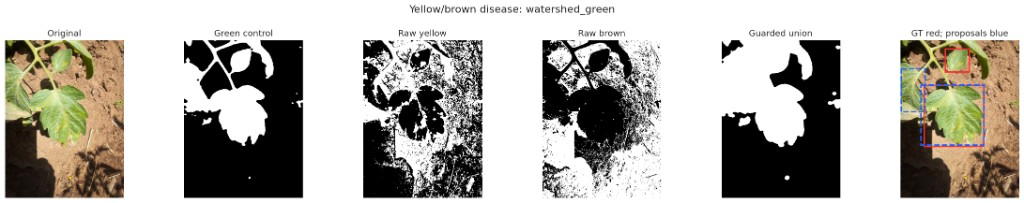
\includegraphics[width=\textwidth]{image/expand_mask_yellow_brown.png}
\caption{A yellow and brown disease photograph. From left: the green control mask, the raw yellow
response, the raw brown response, the guarded union of Section~\ref{sec:expanded-mask}, and the
watershed proposals in blue against the red annotation. The raw responses are mostly scattered
specks, so the guarded union stays close to the control and does not recover the small
annotation.}
\label{fig:expand-yellow}
\end{figure}

\begin{figure}[H]
\centering
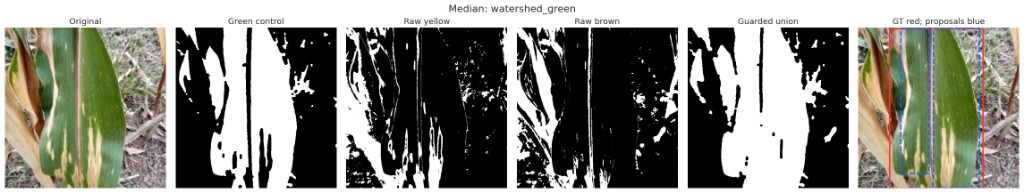
\includegraphics[width=\textwidth]{image/expand_mask_median.png}
\caption{A median-coverage corn leaf. The green control drops the yellow streaks. The guarded
union restores those touching green tissue, so the mask follows more of the leaf. The annotation in
red still covers the whole leaf while the proposals in blue remain partial strips, which is the
pattern that raises mean best IoU without raising the hit rate.}
\label{fig:expand-median}
\end{figure}

\begin{figure}[H]
\centering
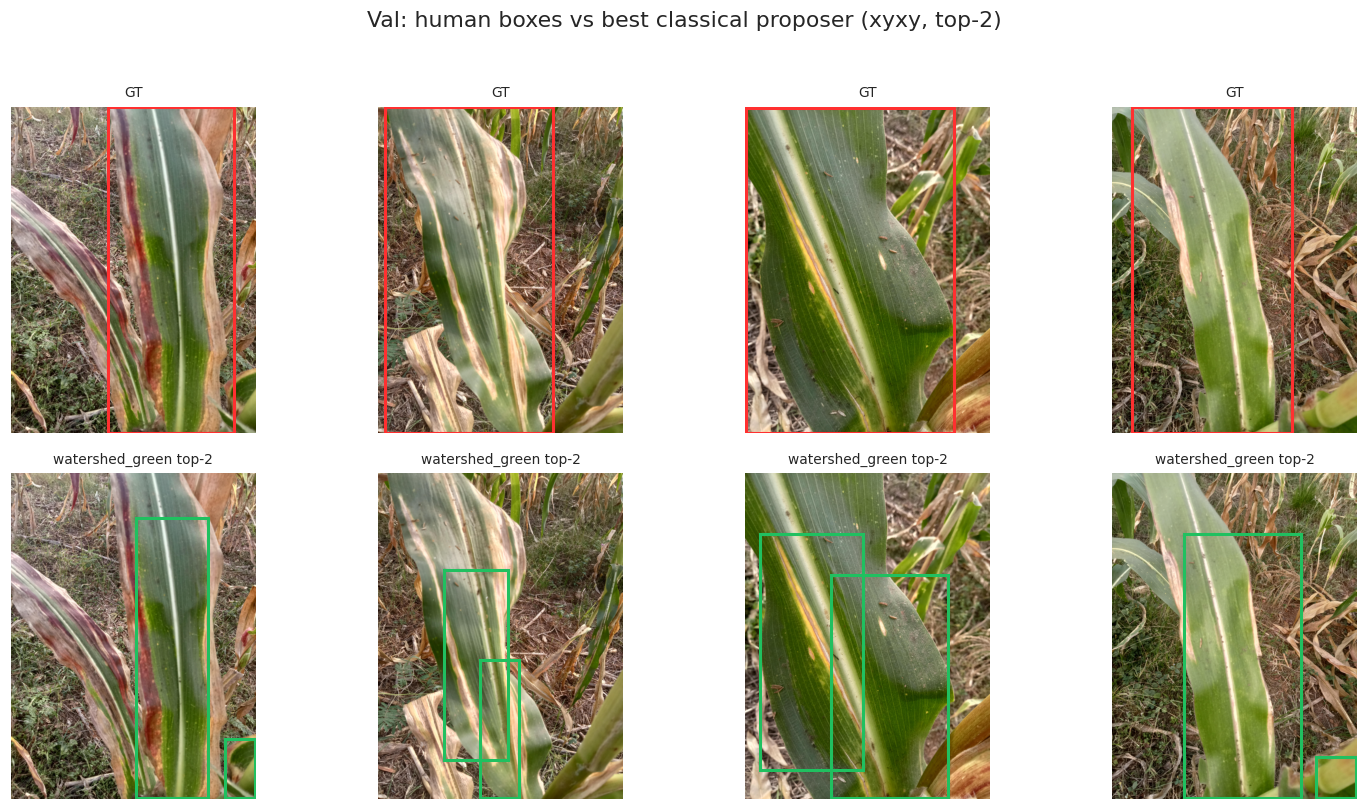
\includegraphics[width=\textwidth]{image/proposal_methods.png}
\caption{Validation examples comparing the annotations in red (top) with the boxes in green
(bottom) produced by the selected configuration, watershed on the green control mask.}
\label{fig:proposal-methods}
\end{figure}

Figure~\ref{fig:proposal-methods} shows merging, fragmentation, shadow responses, and large
background components, explaining the low observed localization coverage.

\subsection{Classification performance on ground-truth crops}
\label{sec:classifier-results}

The classification stage is evaluated first in isolation, on crops taken from the annotations
themselves. This isolates classification from localization and provides a reference for the
proposal-crop evaluation in Section~\ref{sec:attribution}.
Table~\ref{tab:classifiers} compares the three stages.

\begin{table}[H]
\centering
\small
\renewcommand{\arraystretch}{1.2}
\begin{tabularx}{0.97\textwidth}{|>{\raggedright\arraybackslash}X|r|r|r|r|r|}
\hline
\textbf{Stage} & \textbf{Dim.} & \textbf{Macro-$F_1$} & \textbf{Accuracy} & \textbf{Weighted $F_1$} & \textbf{Rare recall}\\
\hline
Basic features, balanced logistic regression & 1{,}812 & 0.324 & 0.589 & 0.593 & 0.091\\
\hline
Enhanced features, balanced logistic regression & 1{,}906 & 0.382 & 0.662 & 0.662 & \textbf{0.200}\\
\hline
Enhanced features, balanced gradient boosting & 1{,}906 & \textbf{0.432} & \textbf{0.778} & \textbf{0.758} & 0.091\\
\hline
\end{tabularx}
\caption{Validation performance on ground-truth crops. Macro-$F_1$ follows
Equation~\eqref{eq:macrof1}, accuracy Equation~\eqref{eq:acc}, weighted $F_1$
Equation~\eqref{eq:weightedf1}, and rare-class recall Equation~\eqref{eq:rarerecall}. The gradient
boosting row is the candidate selected from the grid of Table~\ref{tab:hgb-grid}.}
\label{tab:classifiers}
\end{table}

Enhanced features raise logistic-regression macro-$F_1$ from 0.324 to 0.382, and gradient
boosting raises it to 0.432 with accuracy 0.778. Enhanced logistic regression has higher rare
recall (0.200 versus 0.091), but macro-$F_1$ is the primary criterion, so enhanced gradient
boosting is selected.

\begin{table}[H]
\centering
\small
\renewcommand{\arraystretch}{1.15}
\begin{tabularx}{0.97\textwidth}{|c|c|c|r|r|r|r|X|}
\hline
\textbf{Rate} & \textbf{Leaves} & \textbf{$L_2$} & \textbf{Macro-$F_1$} & \textbf{Accuracy} & \textbf{Rare recall} & \textbf{Fit (s)} & \\
\hline
0.05 & 31 & 1 & \textbf{0.432} & 0.778 & \textbf{0.091} & 109.9 & selected\\
\hline
0.05 & 15 & 0 & 0.423 & 0.780 & 0.000 & 103.9 & \\
\hline
0.10 & 31 & 1 & 0.422 & 0.775 & 0.000 & 113.0 & \\
\hline
0.05 & 15 & 1 & 0.413 & 0.772 & 0.000 & 89.9 & \\
\hline
0.10 & 15 & 1 & 0.412 & 0.778 & 0.000 & 90.4 & \\
\hline
0.05 & 31 & 0 & 0.404 & 0.772 & 0.000 & 158.2 & \\
\hline
0.10 & 31 & 0 & 0.382 & 0.778 & 0.000 & 135.3 & \\
\hline
0.10 & 15 & 0 & 0.366 & 0.773 & 0.000 & 100.2 & \\
\hline
\end{tabularx}
\caption{The eight gradient boosting candidates on validation ground-truth crops, ordered by
macro-$F_1$ then by rare-class recall. All use 100 boosting iterations, at least 20 samples per
leaf, 63 bins, balanced class weights, and no early stopping.}
\label{tab:hgb-grid}
\end{table}

Across Table~\ref{tab:hgb-grid}, accuracy varies only from 0.772 to 0.780 while macro-$F_1$
varies from 0.366 to 0.432. The selected lower-rate, $L_2$-regularized model is also the only
candidate with non-zero median rare-class recall.

\subsection{End-to-end attribution of the classical pipeline}
\label{sec:attribution}

Combining the selected proposer with the selected classifier gives the complete classical system.
Table~\ref{tab:e2e} reports it beside a control in which only the classifier is downgraded, so
that the effect of the proposal stage can be read off directly.

\begin{table}[H]
\centering
\small
\renewcommand{\arraystretch}{1.2}
\begin{tabularx}{\textwidth}{|>{\raggedright\arraybackslash}X|c|r|r|r|r|r|}
\hline
\textbf{Configuration} & \textbf{Split} & \textbf{GT-crop} & \textbf{End-to-end} & \textbf{$\mathrm{HR}_{0.5}$} & \textbf{Matched} & \textbf{Unmatched}\\
\hline
Watershed green, basic logistic regression & val & 0.324 & 0.258 & 32.9\% & 434 & 884\\
\hline
Watershed green, enhanced boosting & val & 0.432 & 0.348 & 32.9\% & 434 & 884\\
\hline
Watershed green, enhanced boosting & test & 0.477 & 0.387 & 30.3\% & 383 & 882\\
\hline
\end{tabularx}
\caption{Classical end-to-end attribution. ``GT-crop'' is macro-$F_1$ on annotation crops, the
reference for the classification stage. ``End-to-end'' is macro-$F_1$ on matched proposal crops.
Unmatched objects are localization false negatives per Equation~\eqref{eq:match} and are
excluded from the proposal-crop score; the GT-crop score evaluates all annotation crops.}
\label{tab:e2e}
\end{table}

On validation, imprecise proposal crops reduce macro-$F_1$ from 0.432 to 0.348. The larger loss is
localization: only \textbf{434 of 1,318 objects} are matched, leaving 884 without any
classification. Test macro-$F_1$ is higher despite a lower 30.3\% hit rate.

\subsection{Detector results}
\label{sec:yolo-results}

\begin{table}[H]
\centering
\small
\renewcommand{\arraystretch}{1.2}
\begin{tabularx}{0.9\textwidth}{|>{\raggedright\arraybackslash}X|r|r|}
\hline
\textbf{Metric} & \textbf{Validation} & \textbf{Test}\\
\hline
$\mathrm{mAP}@0.5$ & 0.695 & 0.744\\
\hline
$\mathrm{mAP}@[0.5{:}0.95]$ & 0.548 & 0.609\\
\hline
Precision & 0.686 & 0.676\\
\hline
Recall & 0.689 & 0.675\\
\hline
Objects & 1{,}318 & 1{,}265\\
\hline
\end{tabularx}
\caption{YOLO26n detection metrics, following Equation~\eqref{eq:map}. Precision and recall are
read at the confidence threshold maximizing $F_1$ and are therefore a single operating point on
the curve that mAP integrates.}
\label{tab:yolo-detection}
\end{table}

The validation gap of 0.147 between $\mathrm{mAP}@0.5$ and
$\mathrm{mAP}@[0.5{:}0.95]$ reflects stricter box fitting. Precision and recall are nearly equal
at the $F_1$-maximizing threshold. Test mAP is 0.049 higher at IoU 0.5.

\begin{figure}[H]
\centering
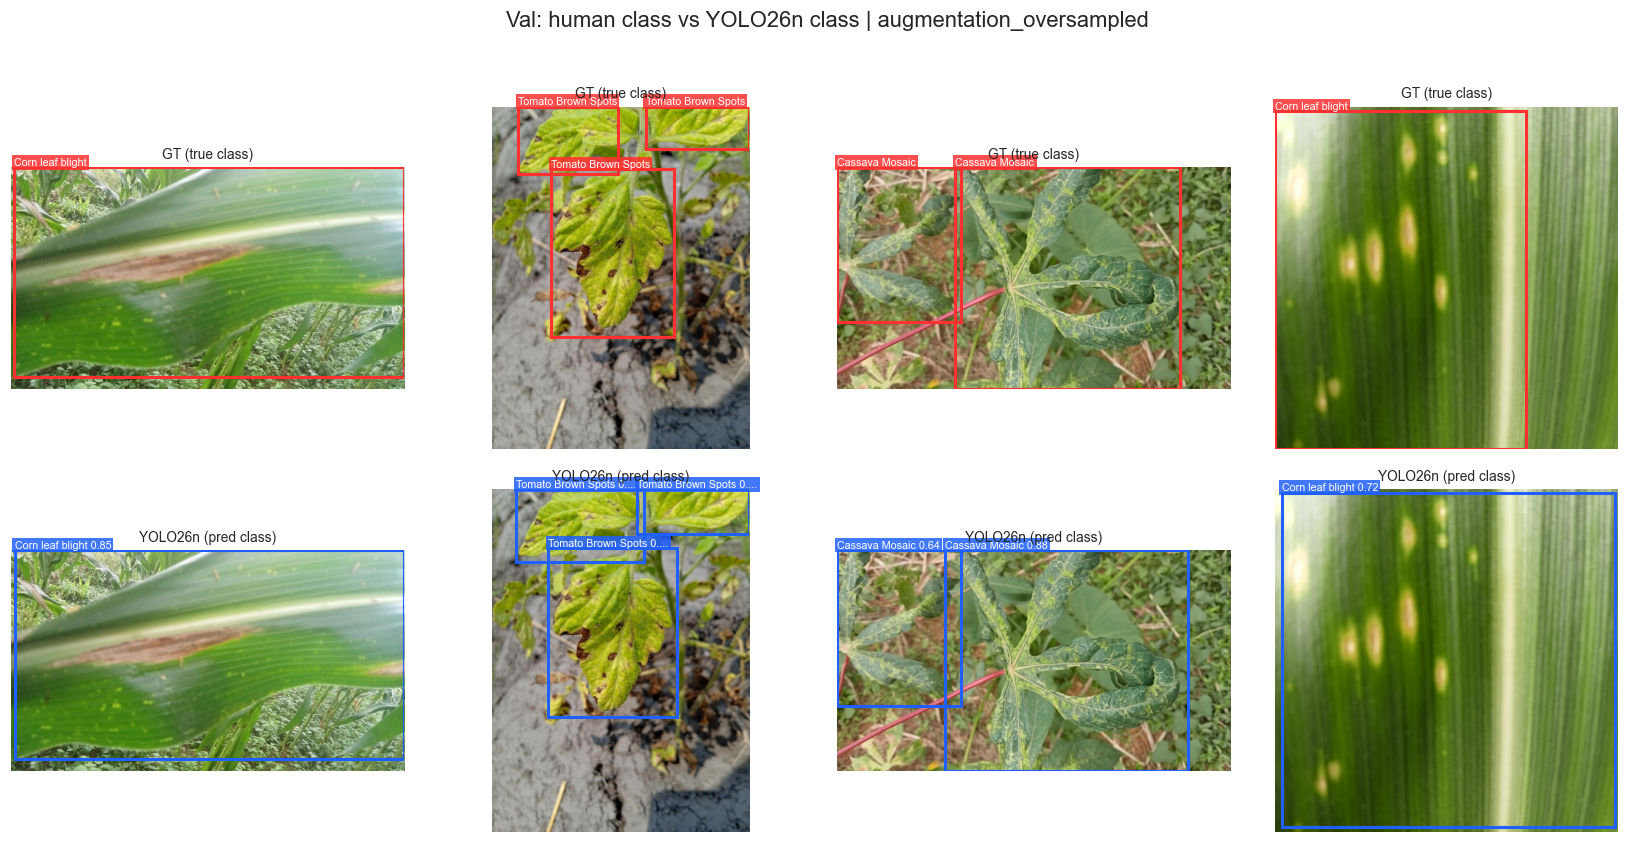
\includegraphics[width=\textwidth]{image/yolo_predictions.png}
\caption{Validation examples with annotations in red and YOLO26n predictions in blue. Numbers
beside the predicted labels are confidence scores. Predictions are filtered at confidence
0.25 before the matching analysis of Section~\ref{sec:parity}. Retained predictions are
matched one-to-one at $\mathrm{IoU} \ge 0.5$; confidence does not weight the matched scores.}
\label{fig:yolo-predictions}
\end{figure}

Figure~\ref{fig:yolo-predictions} shows boxes following object rather than colour boundaries,
including discoloured and adjacent leaves. YOLO26n also has no two-output ceiling.

\subsection{Two tracks comparison}
\label{sec:parity}

The two tracks are now compared under one protocol. Both are matched to the same annotations by
Equation~\eqref{eq:match} at $\tau = 0.5$. YOLO26n predictions are first filtered at a fixed
confidence threshold of 0.25, as in the notebook's parity evaluation. Classical proposals
have no confidence score and use the top-two retention rule. Macro-$F_1$ is computed on
matched pairs only, with the class set defined in Section~\ref{sec:aggregation}; unmatched
objects are excluded from this classification score and reported separately through hit
rate and unmatched counts. Confidence does not weight the matched score, but its filtering
threshold affects which YOLO predictions are available for matching.

\begin{table}[H]
\centering
\small
\renewcommand{\arraystretch}{1.25}
\begin{tabularx}{\textwidth}{|>{\raggedright\arraybackslash}X|r|r|r|r|}
\hline
\textbf{Method} & \textbf{Matched macro-$F_1$} & \textbf{$\mathrm{HR}_{0.5}$} & \textbf{Matched objects} & \textbf{Unmatched objects}\\
\hline
Watershed green proposals with enhanced boosting & 0.348 & 32.9\% & 434 & 884\\
\hline
YOLO26n with augmentation and oversampling & \textbf{0.802} & \textbf{84.4\%} & \textbf{1{,}113} & \textbf{205}\\
\hline
\end{tabularx}
\caption{Validation parity between the two tracks. Matched macro-$F_1$ follows
Equation~\eqref{eq:macrof1} over matched pairs, and hit rate follows
Equation~\eqref{eq:hitrate}. Both are computed over the same 1{,}318 annotated objects.}
\label{tab:parity}
\end{table}

YOLO26n matches \textbf{1,113 of 1,318 objects} versus 434, giving 84.4\% versus 32.9\% hit rate,
and raises matched macro-$F_1$ from 0.348 to 0.802. The joint comparison shows a substantial
increase in both localization coverage and matched classification performance.

\subsection{Error analysis}
\label{sec:error-analysis}

\subsubsection{Failure modes of the classical pipeline}

On annotation crops, \textbf{six of 25 evaluable classes have $F1_c=0$}; all have fewer than 20
training boxes and at most five validation objects. High-scoring classes mainly show broad colour
or pattern changes captured by global histograms, whereas small localized lesions are diluted.
The failures therefore reflect both low support and loss of spatial detail.

\ref{app:perclass} gives the full per-class report.

\subsubsection{Failure modes of the detector}

Tomato leaf mosaic virus is worst, with zero recall and $\mathrm{AP}@0.5=0.091$ over four
validation objects. Four classes reach recall 1.000 on at most four objects each; median
low-support recall is 0.752. There are 510 unmatched predictions. Tomato healthy shows the largest test
regression, plausibly related to its frequent co-occurrence with Tomato blight leaf.

\section{Limitations}
\label{sec:limitations}

\begin{enumerate}
\item \textbf{Dataset coverage and leakage.} The duplicate groups described in
Section~\ref{sec:eda} can inflate held-out performance. The absent classes and sparse support
documented in Section~\ref{sec:imbalance} restrict held-out claims and make rare-class estimates
unstable. Class weighting and repetition cannot create missing variation. Differences between
validation and test scores on this single split do not establish improved generalization.

\item \textbf{Different classification populations.} Proposal-crop macro-$F_1$ excludes unmatched
annotations and predictions and must be read with hit rate and unmatched counts. The two tracks
match different subsets, so their classification scores do not measure performance on identical
objects. Ground-truth-crop scores are a separate reference, not a strict upper bound on scores
from a selected subset. Detection AP also uses a different population and confidence ranking.

\item \textbf{Greedy matching and geometric summaries.} Equation~\eqref{eq:match} may accept
fewer pairs than an optimal bipartite assignment. Although shared, this protocol may affect the
two methods differently. IoU alone also cannot distinguish displacement, size errors, and merged
objects, motivating qualitative error inspection.

\item \textbf{Annotation completeness.} Some unmatched predictions may be unlabelled plants
rather than true false positives; confirming this requires manual annotation review.

\item \textbf{No controlled detector ablations.} The detector uses augmentation and oversampling
together. Without separate ablations, their individual contributions cannot be determined.
\end{enumerate}

\section{Conclusion and Future Work}
\label{sec:conclusion}

\subsection{Conclusion}

FieldPlant is highly imbalanced, and colour-based localization is the main classical bottleneck.
The selected watershed pipeline reaches 32.9\% hit rate and matched macro-$F_1=0.348$, whereas
YOLO26n reaches 84.4\% and 0.802 under the same protocol. YOLO26n also obtains validation
$\mathrm{mAP}@0.5=0.695$. These results favour joint detection for this experiment.

\subsection{Future work}

Future work should rebuild duplicate-safe partitions, compare a learned class-agnostic proposer
with the handcrafted classifier, and run controlled detector ablations for augmentation and
oversampling. Additional data collection should target the ten classes with fewer than 20
training boxes.

\clearpage
\appendix
\renewcommand{\thesection}{Appendix~\Alph{section}}
\section{Per-class Results}
\label{app:perclass}

Table~\ref{tab:classical-report} reports validation performance on annotation crops. Zero-support
rows identify classes absent from held-out data.

\begin{table}[H]
\centering
\scriptsize
\renewcommand{\arraystretch}{1.1}
\begin{tabularx}{0.92\textwidth}{|>{\raggedright\arraybackslash}X|r|r|r|r|}
\hline
\textbf{Class} & \textbf{Precision} & \textbf{Recall} & \textbf{$F1_c$} & \textbf{Support}\\
\hline
Cassava Bacterial Blight & 0.000 & 0.000 & 0.000 & 5\\
Cassava Brown Leaf Spot & 0.556 & 0.294 & 0.385 & 34\\
Cassava Healthy & 0.800 & 0.686 & 0.738 & 70\\
Cassava Mosaic & 0.849 & 0.944 & 0.894 & 285\\
Cassava Root Rot & 0.333 & 0.091 & 0.143 & 11\\
Corn Brown Spots & 0.875 & 0.226 & 0.359 & 31\\
Corn Charcoal & 0.000 & 0.000 & 0.000 & 0\\
Corn Chlorotic Leaf Spot & 0.500 & 0.250 & 0.333 & 4\\
Corn Gray leaf spot & 0.500 & 0.100 & 0.167 & 10\\
Corn Healthy & 0.545 & 0.240 & 0.333 & 25\\
Corn Insects Damages & 0.000 & 0.000 & 0.000 & 3\\
Corn Mildew & 0.714 & 0.833 & 0.769 & 6\\
Corn Purple Discoloration & 0.000 & 0.000 & 0.000 & 1\\
Corn Smut & 0.000 & 0.000 & 0.000 & 2\\
Corn Streak & 0.667 & 0.571 & 0.615 & 35\\
Corn Stripe & 0.840 & 0.840 & 0.840 & 25\\
Corn Violet Decoloration & 0.000 & 0.000 & 0.000 & 1\\
Corn Yellow Spots & 1.000 & 0.333 & 0.500 & 3\\
Corn Yellowing & 0.753 & 0.773 & 0.763 & 75\\
Corn leaf blight & 0.677 & 0.875 & 0.763 & 256\\
Corn rust leaf & 0.667 & 0.571 & 0.615 & 7\\
Tomato Brown Spots & 0.924 & 0.943 & 0.934 & 298\\
Tomato bacterial wilt & 0.000 & 0.000 & 0.000 & 0\\
Tomato blight leaf & 0.597 & 0.694 & 0.642 & 62\\
Tomato healthy & 0.600 & 0.349 & 0.441 & 43\\
Tomato leaf mosaic virus & 0.000 & 0.000 & 0.000 & 4\\
Tomato leaf yellow virus & 0.647 & 0.500 & 0.564 & 22\\
\hline
\textbf{Accuracy} & \multicolumn{3}{c|}{0.778} & 1{,}318\\
\hline
\textbf{Macro average (27 rows)} & 0.483 & 0.375 & 0.400 & 1{,}318\\
\hline
\textbf{Weighted average} & 0.764 & 0.778 & 0.758 & 1{,}318\\
\hline
\end{tabularx}
\caption{Per-class validation performance of enhanced features with balanced gradient boosting on
ground-truth crops, following Equation~\eqref{eq:prf}. Macro averages follow
Equation~\eqref{eq:macrof1}: over the 25 evaluable classes the macro-$F_1$ is $0.432$, and over all
27 rows it is $0.400$.}
\label{tab:classical-report}
\end{table}

Table~\ref{tab:yolo-perclass} reports both held-out partitions for the 25 evaluable classes.

\begin{table}[H]
\centering
\scriptsize
\renewcommand{\arraystretch}{1.1}
\begin{tabularx}{\textwidth}{|>{\raggedright\arraybackslash}X|r|r|r|r||r|r|r|r|}
\hline
& \multicolumn{4}{c||}{\textbf{Validation}} & \multicolumn{4}{c|}{\textbf{Test}}\\
\cline{2-9}
\textbf{Class} & \textbf{$n$} & \textbf{$P$} & \textbf{$R$} & \textbf{AP50} &
\textbf{$n$} & \textbf{$P$} & \textbf{$R$} & \textbf{AP50}\\
\hline
Cassava Bacterial Blight & 5 & 0.281 & 0.400 & 0.209 & 3 & 0.222 & 0.333 & 0.178\\
Cassava Brown Leaf Spot & 34 & 0.724 & 0.471 & 0.649 & 29 & 0.730 & 0.724 & 0.762\\
Cassava Healthy & 70 & 0.724 & 0.743 & 0.836 & 57 & 0.852 & 0.707 & 0.820\\
Cassava Mosaic & 285 & 0.766 & 0.811 & 0.855 & 284 & 0.791 & 0.771 & 0.840\\
Cassava Root Rot & 11 & 0.516 & 0.636 & 0.538 & 12 & 0.849 & 0.472 & 0.575\\
Corn Brown Spots & 31 & 0.696 & 0.516 & 0.575 & 33 & 0.811 & 0.788 & 0.775\\
Corn Chlorotic Leaf Spot & 4 & 0.645 & 1.000 & 0.787 & 4 & 0.561 & 0.750 & 0.808\\
Corn Gray leaf spot & 10 & 0.484 & 0.600 & 0.628 & 8 & 0.620 & 0.500 & 0.660\\
Corn Healthy & 25 & 0.506 & 0.600 & 0.585 & 19 & 0.581 & 0.579 & 0.666\\
Corn Insects Damages & 3 & 0.489 & 0.667 & 0.696 & 2 & 0.291 & 0.500 & 0.662\\
Corn Mildew & 6 & 0.604 & 0.833 & 0.640 & 6 & 0.484 & 0.833 & 0.749\\
Corn Purple Discoloration & 1 & 0.754 & 1.000 & 0.995 & 1 & 0.696 & 1.000 & 0.995\\
Corn Smut & 2 & 0.943 & 0.500 & 0.551 & 2 & 0.717 & 0.500 & 0.495\\
Corn Streak & 35 & 0.845 & 0.624 & 0.778 & 41 & 0.848 & 0.680 & 0.793\\
Corn Stripe & 25 & 0.694 & 0.635 & 0.688 & 24 & 0.841 & 0.625 & 0.764\\
Corn Violet Decoloration & 1 & 0.364 & 1.000 & 0.995 & 1 & 0.677 & 1.000 & 0.995\\
Corn Yellow Spots & 3 & 0.839 & 1.000 & 0.995 & 2 & 0.575 & 0.500 & 0.828\\
Corn Yellowing & 75 & 0.884 & 0.710 & 0.799 & 73 & 0.847 & 0.671 & 0.855\\
Corn leaf blight & 256 & 0.821 & 0.574 & 0.755 & 239 & 0.810 & 0.669 & 0.800\\
Corn rust leaf & 7 & 0.690 & 0.857 & 0.682 & 9 & 0.887 & 0.877 & 0.918\\
Tomato Brown Spots & 298 & 0.796 & 0.851 & 0.916 & 302 & 0.787 & 0.844 & 0.903\\
Tomato blight leaf & 62 & 0.731 & 0.758 & 0.782 & 62 & 0.878 & 0.806 & 0.900\\
Tomato healthy & 43 & 0.547 & 0.698 & 0.604 & 33 & 0.328 & 0.333 & 0.276\\
Tomato leaf mosaic virus & 4 & 1.000 & 0.000 & 0.091 & 3 & 0.514 & 0.667 & 0.753\\
Tomato leaf yellow virus & 22 & 0.805 & 0.752 & 0.756 & 16 & 0.702 & 0.750 & 0.821\\
\hline
\textbf{All classes} & 1{,}318 & 0.686 & 0.689 & 0.695 & 1{,}265 & 0.676 & 0.675 & 0.744\\
\hline
\end{tabularx}
\caption{YOLO26n per-class precision, recall, and $\mathrm{AP}@0.5$ on validation and test,
following Equations~\eqref{eq:det-pr} and~\eqref{eq:ap}. These detection metrics include unmatched
detections and annotations, unlike matched-only classification. Support is the number of annotated objects of
that class in the partition.}
\label{tab:yolo-perclass}
\end{table}

Table~\ref{tab:tiers} gives the training-count multiplier and resulting effective count.

\begin{table}[H]
\centering
\scriptsize
\renewcommand{\arraystretch}{1.08}
\begin{tabularx}{0.95\textwidth}{|X|r|c|r||X|r|c|r|}
\hline
\textbf{Class} & \textbf{Boxes} & \textbf{$m$} & \textbf{Eff.} &
\textbf{Class} & \textbf{Boxes} & \textbf{$m$} & \textbf{Eff.}\\
\hline
Cassava Bacterial Blight & 17 & 3 & 51 & Corn Streak & 176 & 1 & 176\\
Cassava Brown Leaf Spot & 148 & 1 & 148 & Corn Stripe & 113 & 1 & 113\\
Cassava Healthy & 290 & 1 & 290 & Corn Violet Decoloration & 5 & 4 & 20\\
Cassava Mosaic & 1{,}328 & 1 & 1{,}328 & Corn Yellow Spots & 11 & 3 & 33\\
Cassava Root Rot & 54 & 2 & 108 & Corn Yellowing & 347 & 1 & 347\\
Corn Brown Spots & 156 & 1 & 156 & Corn leaf blight & 1{,}157 & 1 & 1{,}157\\
Corn Charcoal & 1 & 4 & 4 & Corn rust leaf & 33 & 2 & 66\\
Corn Chlorotic Leaf Spot & 18 & 3 & 54 & Tomato Brown Spots & 1{,}367 & 1 & 1{,}367\\
Corn Gray leaf spot & 36 & 2 & 72 & Tomato bacterial wilt & 2 & 4 & 8\\
Corn Healthy & 108 & 1 & 108 & Tomato blight leaf & 280 & 1 & 280\\
Corn Insects Damages & 12 & 3 & 36 & Tomato healthy & 203 & 1 & 203\\
Corn Mildew & 31 & 2 & 62 & Tomato leaf mosaic virus & 12 & 3 & 36\\
Corn Purple Discoloration & 6 & 4 & 24 & Tomato leaf yellow virus & 77 & 2 & 154\\
Corn Smut & 9 & 4 & 36 & & & & \\
\hline
\end{tabularx}
\caption{Class-aware repetition tiers from Equation~\eqref{eq:tiers} and the resulting effective
training box counts. The manifest expands 3{,}609 image paths to 3{,}984 entries.}
\label{tab:tiers}
\end{table}

\section{Computational Environment}
\label{app:repro}

\begin{table}[H]
\centering
\small
\renewcommand{\arraystretch}{1.2}
\begin{tabularx}{0.95\textwidth}{|l|>{\raggedright\arraybackslash}X|}
\hline
\textbf{Item} & \textbf{Value}\\
\hline
Python & 3.12.13\\
\hline
Detection framework & Ultralytics 8.4.163~\cite{yolo26} with PyTorch 2.10.0+cu128\\
\hline
Classical stack & OpenCV, scikit-image, scikit-learn, NumPy, pandas\\
\hline
Accelerator & One NVIDIA Tesla T4, 14{,}912\,MiB\\
\hline
\end{tabularx}
\caption{Software and hardware environment of the reported run.}
\label{tab:repro}
\end{table}

\clearpage
\addcontentsline{toc}{section}{References}
\begin{thebibliography}{99}

\bibitem{fieldplant} E. Moupojou, A. Tagne, F. Retraint, A. Tadonkemwa, D. Wilfried, H. Tapamo, and M. Nkenlifack, ``FieldPlant: A Dataset of Field Plant Images for Plant Disease Detection and Classification With Deep Learning,'' \textit{IEEE Access}, vol.~11, pp.~35398--35410, 2023. \url{https://doi.org/10.1109/ACCESS.2023.3263042}

\bibitem{roboflow} Roboflow Universe, FieldPlant object-detection dataset. \url{https://universe.roboflow.com/plant-disease-detection/fieldplant}

\bibitem{yolo26} G. Jocher, J. Qiu, M. Liu, S. Lyu, F.~C. Akyon, and M.~E. Kalfaoglu, ``Ultralytics YOLO26: Unified Real-Time End-to-End Vision Models,'' arXiv:2606.03748, 2026. The nano detection model used in this report is YOLO26n. \url{https://arxiv.org/abs/2606.03748}

\end{thebibliography}
\end{document}
